%==============================================================================
% Tento soubor použijte jako základ
% This file should be used as a base for the thesis
% Autoři / Authors: 2008 Michal Bidlo, 2022 Jaroslav Dytrych, 2025 Petr Veigend
% Kontakt pro dotazy a připomínky: sablona@fit.vutbr.cz
% Contact for questions and comments: sablona@fit.vutbr.cz
%==============================================================================
% kódování: UTF-8 (zmena prikazem iconv, recode nebo cstocs)
% encoding: UTF-8 (you can change it by command iconv, recode or cstocs)
%------------------------------------------------------------------------------
% zpracování / processing: make, make pdf, make clean
%==============================================================================
% Soubory, které je nutné upravit nebo smazat: / Files which have to be edited or deleted:
%   projekt-20-literatura-bibliography.bib - literatura / bibliography
%   projekt-01-kapitoly-chapters.tex - obsah práce / the thesis content
%   projekt-01-kapitoly-chapters-en.tex - obsah práce v angličtině / the thesis content in English
%   projekt-30-prilohy-appendices.tex - přílohy / appendices
%   projekt-30-prilohy-appendices-en.tex - přílohy v angličtině / appendices in English
%==============================================================================
%\documentclass[]{fitthesis} % bez zadání - pro začátek práce, aby nebyl problém s překladem
% \documentclass[english]{fitthesis} % without assignment - for the work start to avoid compilation problem
%\documentclass[zadani]{fitthesis} % odevzdani do IS VUT a/nebo tisk s barevnými odkazy - odkazy jsou barevné
% \documentclass[english,zadani]{fitthesis} % for submission to the IS VUT and/or print with color links - links are color
%\documentclass[zadani,print]{fitthesis} % pro černobílý tisk - odkazy jsou černé
%\documentclass[english,zadani,print]{fitthesis} % for the black and white print - links are black
%\documentclass[zadani,cprint]{fitthesis} % pro barevný tisk - odkazy jsou černé, znak VUT barevný
\documentclass[english,zadani,cprint]{fitthesis} % for the print - links are black, logo is color
% * Je-li práce psaná v anglickém jazyce, je zapotřebí u třídy použít 
%   parametr english následovně:
%   If thesis is written in English, it is necessary to use 
%   parameter english as follows:
%      \documentclass[english]{fitthesis}
% * Je-li práce psaná ve slovenském jazyce, je zapotřebí u třídy použít 
%   parametr slovak následovně:
%   If the work is written in the Slovak language, it is necessary 
%   to use parameter slovak as follows:
%      \documentclass[slovak]{fitthesis}
% * Je-li práce psaná v anglickém jazyce se slovenským abstraktem apod., 
%   je zapotřebí u třídy použít parametry english a enslovak následovně:
%   If the work is written in English with the Slovak abstract, etc., 
%   it is necessary to use parameters english and enslovak as follows:
%      \documentclass[english,enslovak]{fitthesis}

% Základní balíčky jsou dole v souboru šablony fitthesis.cls
% Basic packages are at the bottom of template file fitthesis.cls
% zde můžeme vložit vlastní balíčky / you can place own packages here


% Pro seznam zkratek lze využít balíček Glossaries - nutno odkomentovat i níže a při kompilaci z konzoly i v Makefile (plnou verzi pro Perl, nebo lite)
% The Glossaries package can be used for the list of abbreviations - it is necessary to uncomment also below. When compiling from the console also in the Makefile (full version for Perl or lite)
%\usepackage{glossaries}
%\usepackage{glossary-superragged}
%\makeglossaries 

% Nastavení cesty k obrázkům
% Setting of a path to the pictures
%\graphicspath{{obrazky-figures/}{./obrazky-figures/}}
%\graphicspath{{obrazky-figures/}{../obrazky-figures/}}

%---rm---------------
\renewcommand{\rmdefault}{lmr}%zavede Latin Modern Roman jako rm / set Latin Modern Roman as rm
%---sf---------------
\renewcommand{\sfdefault}{qhv}%zavede TeX Gyre Heros jako sf
%---tt------------
\renewcommand{\ttdefault}{lmtt}% zavede Latin Modern tt jako tt

% vypne funkci šablony, která automaticky nahrazuje uvozovky,
% aby nebyly prováděny nevhodné náhrady v popisech API apod.
% disables function of the template which replaces quotation marks
% to avoid unnecessary replacements in the API descriptions etc.
\csdoublequotesoff

\usepackage{url}

% =======================================================================
% balíček "hyperref" vytváří klikací odkazy v pdf, pokud tedy použijeme pdflatex
% problém je, že balíček hyperref musí být uveden jako poslední, takže nemůže
% být v šabloně
% "hyperref" package create clickable links in pdf if you are using pdflatex.
% Problem is that this package have to be introduced as the last one so it 
% can not be placed in the template file.
\ifWis
\ifx\pdfoutput\undefined % nejedeme pod pdflatexem / we are not using pdflatex
\else
  \usepackage{color}
  \usepackage[unicode,colorlinks,hyperindex,plainpages=false,pdftex]{hyperref}
  \definecolor{hrcolor-ref}{RGB}{223,52,30}
  \definecolor{hrcolor-cite}{HTML}{2F8F00}
  \definecolor{hrcolor-urls}{HTML}{092EAB}
  \hypersetup{
	linkcolor=hrcolor-ref,
	citecolor=hrcolor-cite,
	filecolor=magenta,
	urlcolor=hrcolor-urls
  }
  \def\pdfBorderAttrs{/Border [0 0 0] }  % bez okrajů kolem odkazů / without margins around links
  \pdfcompresslevel=9
\fi
\else % pro tisk budou odkazy, na které se dá klikat, černé / for the print clickable links will be black
\ifx\pdfoutput\undefined % nejedeme pod pdflatexem / we are not using pdflatex
\else
  \usepackage{color}
  \usepackage[unicode,colorlinks,hyperindex,plainpages=false,pdftex,urlcolor=black,linkcolor=black,citecolor=black]{hyperref}
  \definecolor{links}{rgb}{0,0,0}
  \definecolor{anchors}{rgb}{0,0,0}
  \def\AnchorColor{anchors}
  \def\LinkColor{links}
  \def\pdfBorderAttrs{/Border [0 0 0] } % bez okrajů kolem odkazů / without margins around links
  \pdfcompresslevel=9
\fi
\fi
% Řešení problému, kdy klikací odkazy na obrázky vedou za obrázek
% This solves the problems with links which leads after the picture
\usepackage[all]{hypcap}


% Informace o práci/projektu / Information about the thesis
%---------------------------------------------------------------------------
\projectinfo{
  %Prace / Thesis
  project={BP},            %typ práce BP/SP/DP/DR  / thesis type (SP = term project)
  year={2026},             % rok odevzdání / year of submission
  date=\today,             % datum odevzdání / submission date
  %Nazev prace / thesis title
  title.cs={Implementace výstupů strojového učení na vestavných platformách},  % název práce v češtině či slovenštině (dle zadání) / thesis title in czech language (according to assignment)
  title.en={Implementation of Machine Learning Outputs on Embedded Platforms}, % název práce v angličtině / thesis title in english
  title.length={13.5cm}, % nastavení délky bloku s titulkem pro úpravu zalomení řádku (lze definovat zde nebo níže) / setting the length of a block with a thesis title for adjusting a line break (can be defined here or below)
  %sectitle.length={14.5cm}, % nastavení délky bloku s druhým titulkem pro úpravu zalomení řádku (lze definovat zde nebo níže) / setting the length of a block with a second thesis title for adjusting a line break (can be defined here or below)
  %dectitle.length={14.5cm}, % nastavení délky bloku s titulkem nad prohlášením pro úpravu zalomení řádku (lze definovat zde nebo níže) / setting the length of a block with a thesis title above declaration for adjusting a line break (can be defined here or below)
  %Autor / Author
  author.name={Daria},   % jméno autora / author name
  author.surname={Kinash},   % příjmení autora / author surname 
  %author.title.p={Bc.}, % titul před jménem (nepovinné) / title before the name (optional)
  %author.title.a={Ph.D.}, % titul za jménem (nepovinné) / title after the name (optional)
  %Ustav / Department
  department={UPSY}, % doplňte příslušnou zkratku dle ústavu na zadání: UPSY/UIFS/UITS/UPGM / fill in appropriate abbreviation of the department according to assignment: UPSY/UIFS/UITS/UPGM
  % Školitel / supervisor
  supervisor.name={Josef},   % jméno školitele / supervisor name 
  supervisor.surname={Strnadel},   % příjmení školitele / supervisor surname
  supervisor.title.p={Ing.},   %titul před jménem (nepovinné) / title before the name (optional)
  supervisor.title.a={Ph.D.},    %titul za jménem (nepovinné) / title after the name (optional)
  % Školitel specialista / Supervisor specialist
  % Vyplňuje se pouze u pojednání disertační práce nebo u disertační práce, pokud existuje školitel specialista. Pokud nemáte školitele specialistu, jméno a příjmení ponechte prázdné. / Is used only with PhD. thesis or proposal. if you have the specialist. If you do not have a specialist, leave name and surname blank.  
  specialist.name={},   % jméno školitele specialisty / supervisor specialist name 
  specialist.surname={},   % příjmení školitele specialisty / supervisor specialist surname
  specialist.title.p={},   %titul před jménem (nepovinné) / title before the name (optional)
  specialist.title.a={},    %titul za jménem (nepovinné) / title after the name (optional)
  % Klíčová slova / keywords
  keywords.cs={strojové učení, vestavěné systémy, mikrokontrolér, TinyML, TensorFlow Lite Micro, LiteRT, rozpoznávání gest, jednorozměrná konvoluční neuronová síť, kvantizace, NXP i.MX RT1050, inerciální měřicí jednotka}, % klíčová slova v českém či slovenském jazyce / keywords in czech or slovak language
  keywords.en={machine learning, embedded systems, microcontroller, TinyML, TensorFlow Lite Micro, LiteRT, gesture recognition, 1D convolutional neural network, quantisation, NXP i.MX RT1050, inertial measurement unit}, % klíčová slova v anglickém jazyce / keywords in english
  %keywords.en={Here, individual keywords separated by commas will be written in English.},
  % Abstrakt / Abstract
  abstract.cs={
  Nasazení strojového učení na mikrokontrolérech umožňuje inferenci v reálném čase bez potřeby síťového připojení, ale vyžaduje pečlivá návrhová rozhodnutí. Tato práce představuje kompletní implementaci strojového učení pro rozpoznávání gest zápěstí v reálném čase na mikrokontroléru NXP~i.MX~RT1050. Kompaktní jednorozměrná konvoluční neuronová síť a pět klasických klasifikátorů byly natrénovány, kvantizovány a nasazeny na cílovém hardwaru a hodnoceny z hlediska přesnosti, latence inference a paměťových nároků. Základní CNN dosáhla přesnosti 94.3\,\% na vlastním datasetu se dvěma subjekty. Plná int8 kvantizace snížila spotřebu SRAM o 75\,\% při změně přesnosti pouze o $+0.4$ procentního bodu a průměrná doba inference na zařízení je 13\,199\,$\mu$s, což je méně než 2\,\% dostupného časového rozpočtu. Mezi klasickými modely dosáhl rozhodovací strom nejrychlejší inference (221\,$\mu$s) při využití méně než 10\,KB flash paměti. Studie hyperparametrů na benchmarku UCI Human Activity Recognition potvrdila správnost navrženého postupu a ukázala, že optimální nastavení se výrazně liší mezi velkými a malými datasety. Na datasetu gest se dvěma subjekty dosahuje logistická regrese stejné přesnosti jako nejlepší CNN, zatímco testování mezi subjekty dosáhlo pouze 34.7\,\% přesnosti, což ukazuje omezenou velikost trénovacích dat jako hlavní limit.}, % abstrakt v českém či slovenském jazyce / abstract in czech or slovak language
  abstract.en={
  Deploying machine learning on microcontrollers enables real-time inference without connectivity, but requires careful design choices. This thesis presents an end-to-end implementation of machine learning for real-time wrist gesture recognition on the NXP~i.MX~RT1050 microcontroller. A compact one-dimensional convolutional neural network and five classical classifiers were trained, quantized, deployed on the target hardware, and evaluated for accuracy, inference latency, and memory consumption. The baseline CNN achieved 94.3\,\% test accuracy on a custom two-subject dataset. Full int8 quantization reduced SRAM consumption by 75\,\% with an accuracy change of only $+0.4$ percentage points, and average on-board inference time is 13\,199\,$\mu$s, under 2\,\% of the available time budget. Among the classical models the decision tree achieved the fastest inference (221\,$\mu$s) with under 10\,KB of flash. A hyperparameter study on the UCI Human Activity Recognition benchmark validated the pipeline and showed that optimal settings differ between large and small datasets. On the two-subject gesture data, logistic regression matches the best CNN result, while cross-subject testing yielded only 34.7\,\% accuracy, identifying the small training corpus as the main limitation.},
  % abstrakt v anglickém jazyce / abstract in english
  %abstract.en={An abstract of the work in English will be written in this paragraph.},
  % Prohlášení (u anglicky psané práce anglicky, u slovensky psané práce slovensky; u projektové praxe lze zakomentovat). Pokud použijete nástroje umělé inteligence, uveďte je podobně jako v příkladu. / Declaration (for thesis in english should be in english; for project practice can be commented out). If you use any AI tools, acknowledge them like in the provided example.
  % declaration={Prohlašuji, že jsem tuto bakalářskou práci vypracovala samostatně pod vedením pana Ing.~Josefa Strnadela, Ph.D. Uvedla jsem všechny literární prameny, publikace a další zdroje, ze kterých jsem čerpala. Pro jazykovou revizi technické zprávy jsem použila nástroj ChatGPT, Claude.},
  declaration={I hereby declare that this Bachelor's thesis was prepared as an original work by the author under the supervision of Ing.~Josef Strnadel, Ph.D. I have listed all the literary sources, publications and other sources, which were used during the preparation of this thesis. I have used ChatGPT and Claude to correct spelling and other language mistakes. },
  % Poděkování (nepovinné, nejlépe v jazyce práce; nechcete-li, zakomentujte pro skrytí nadpisu. / Acknowledgement (optional, ideally in the language of the thesis; comment out to hide it including a heading.) 
  acknowledgment={I would like to sincerely thank my supervisor, Ing.~Josef Strnadel, Ph.D., for his guidance, valuable advice and feedback throughout the writing of this thesis. His consultations and support were essential for both the technical part and the final form of the text.},
  %acknowledgment={Here it is possible to express thanks to the supervisor and to the people which provided professional help
%(external submitter, consultant, etc.).},
  % Rozšířený abstrakt (cca 3 normostrany) - lze definovat zde nebo níže / Extended abstract (approximately 3 standard pages) - can be defined here or below
  %extendedabstract={Do tohoto odstavce bude zapsán rozšířený výtah (abstrakt) práce v českém (slovenském) jazyce.},
  %extabstract.odd={true}, % Začít rozšířený abstrakt na liché stránce? / Should extended abstract start on the odd page?
  %faculty={FIT}, % FIT/FEKT/FSI/FA/FCH/FP/FAST/FAVU/USI/DEF
  faculty.cs={Fakulta informačních technologií}, % Fakulta v češtině - pro využití této položky výše zvolte fakultu DEF / Faculty in Czech - for use of this entry select DEF above
  faculty.en={Faculty of Information Technology}, % Fakulta v angličtině - pro využití této položky výše zvolte fakultu DEF / Faculty in English - for use of this entry select DEF above
  department.cs={Ústav počítačových systémů}, % Ústav v češtině - pro využití této položky výše zvolte ústav DEF nebo jej zakomentujte / Department in Czech - for use of this entry select DEF above or comment it out
  department.en={Department of Computer Systems} % Ústav v angličtině - pro využití této položky výše zvolte ústav DEF nebo jej zakomentujte / Department in English - for use of this entry select DEF above or comment it out
}

% Rozšířený abstrakt (cca 3 normostrany) - lze definovat zde nebo výše / Extended abstract (approximately 3 standard pages) - can be defined here or above
\extendedabstract{Moderní mikrokontroléry dosáhly výkonu, který před několika lety ještě nebyl dostupný ani ve středních embedded systémech. To otevřelo novou třídu aplikací: místo odesílání senzorových dat do cloudu a čekání na odpověď je nyní možné provést celou klasifikaci strojovým učením přímo na čipu v reálném čase. Výhody jsou praktické — nižší latence odezvy, nezávislost na síti, menší spotřeba energie při přenosu dat a zachování soukromí uživatele. Nasazení strojového učení na mikrokontrolérech přesto zůstává technicky náročnou úlohou, která vyžaduje pečlivá rozhodnutí ohledně architektury modelu, kvantizace a optimalizace pro konkrétní hardware.

V rámci této práce byl od základu vybudován celý řetězec strojového učení pro roz\-poz\-n\'{a}\-v\'{a}\-n\'{i} gest zápěstí na mikrokontroléru NXP~i.MX~RT1050. Senzorová data byla sbírána pomocí inerciálního senzoru MPU-6050 od dvou subjektů v opakovaných sezeních. Data byla použita pro trénink kompaktní jednorozměrné konvoluční neuronové sítě v Keras. Model byl kvantizován a nasazen jako firmware pod FreeRTOS přes TFLite Micro. Paralelně bylo implementováno a nasazeno pět klasických klasifikátorů — logistická regrese, SVM, rozhodovací strom, $k$-NN a náhodný les — pracujících na statistickém vektoru příznaků a exportovaných jako C hlavičkové soubory. Všechny modely byly vyhodnoceny z hlediska přesnosti, latence inference a paměťových nároků.

Základní CNN dosáhla na dvousubjektovém datasetu gest přesnosti 94{,}3\,\%; prodloužení vstupního okna ze 100 na 200 vzorků ji zvýšilo na 96{,}2\,\%. Plná int8 kvantizace přinesla výrazné úspory bez znatelné ztráty kvality: spotřeba SRAM klesla o 75\,\% — z 151\,860 na 38\,406 bajtů — zatímco přesnost se změnila o pouhé $+0{,}4$\,p.b. Průměrná latence int8 modelu na desce je 13\,199\,$\mu$s, maximální pak 23\,737\,$\mu$s, obě hodnoty jsou výrazně pod hranicí 1\,000\,ms danou intervalem mezi okny. Model tedy běží v reálném čase s dostatečnou rezervou. Mezi klasickými modely dosáhl rozhodovací strom nejrychlejší inference (221\,$\mu$s) při využití méně než 10\,KB flash paměti. Logistická regrese na vlastním datasetu dosáhla přesnosti 96{,}1\,\% — shodně s nejlepší CNN — což ukazuje, že neuronová síť nepřináší výhodu automaticky, ale jen tehdy, když je k dispozici dostatečné množství a rozmanitost trénovacích dat. Testování přenositelnosti modelu na subjektu nezahrnutém do tréninku dosáhlo přesnosti pouze 34{,}7\,\%, což identifikuje omezený počet trénovacích subjektů jako hlavní omezení systému.

Před aplikací pipeline na vlastní datovou sadu byla provedena studie hyperparametrů na veřejném benchmarku UCI Human Activity Recognition s 30 subjekty, která sloužila jako validační krok ověřující správnost implementace. Studie odhalila prakticky relevantní pozorování: optimální hodnoty rychlosti učení, míry dropoutu a dávkové normalizace se mezi oběma datovými sadami výrazně liší a u několika parametrů se směr efektu obrátí.}
% Začít rozšířený abstrakt na liché stránce? / Should extended abstract start on the odd page?
%\extabstractodd{true}

% nastavení délky bloku s titulkem pro úpravu zalomení řádku - lze definovat zde nebo výše / setting the length of a block with a thesis title for adjusting a line break - can be defined here or above
%\titlelength{14.5cm}
% nastavení délky bloku s druhým titulkem pro úpravu zalomení řádku - lze definovat zde nebo výše / setting the length of a block with a second thesis title for adjusting a line break - can be defined here or above
%\sectitlelength{14.5cm}
% nastavení délky bloku s titulkem nad prohlášením pro úpravu zalomení řádku - lze definovat zde nebo výše / setting the length of a block with a thesis title above declaration for adjusting a line break - can be defined here or above
%\dectitlelength{14.5cm}

% řeší první/poslední řádek odstavce na předchozí/následující stránce
% solves first/last row of the paragraph on the previous/next page
\clubpenalty=10000
\widowpenalty=10000

% checklist
\newlist{checklist}{itemize}{1}
\setlist[checklist]{label=$\square$}

% Kompilace po částech (rychlejší, ale v náhledu nemusí být vše aktuální)
% Compilation piecewise (faster, but not all parts in preview will be up-to-date)
% Další informace viz / For more information see https://www.overleaf.com/learn/latex/Multi-file_LaTeX_projects
% \usepackage{subfiles}

% Nechcete-li, aby se u oboustranného tisku roztahovaly mezery pro zaplnění stránky, odkomentujte následující řádek / If you do not want enlarged spacing for filling of the pages in case of duplex printing, uncomment the following line
% \raggedbottom

\begin{document}
  % Vysazeni titulnich stran / Typesetting of the title pages
  % ----------------------------------------------
  \maketitle
  % Obsah
  % ----------------------------------------------
  \setlength{\parskip}{0pt}

  {\hypersetup{hidelinks}\tableofcontents}
  
  % Seznam obrazku a tabulek (pokud prace obsahuje velke mnozstvi obrazku, tak se to hodi)
  % List of figures and list of tables (if the thesis contains a lot of pictures, it is good)
  \ifczech
    \renewcommand\listfigurename{Seznam obrázků}
  \fi
  \ifslovak
    \renewcommand\listfigurename{Zoznam obrázkov}
  \fi
  {\hypersetup{hidelinks}\listoffigures}
  
  \ifczech
    \renewcommand\listtablename{Seznam tabulek}
  \fi
  \ifslovak
    \renewcommand\listtablename{Zoznam tabuliek}
  \fi
  {\hypersetup{hidelinks}\listoftables}

  % Seznam zkratek / List of abbreviations
  %\ifczech
  %  \renewcommand*\glossaryname{Seznam zkratek}%
  %  \renewcommand*\entryname{Zkratka}
  %  \renewcommand*\descriptionname{Význam}
  %\fi
  %\ifslovak
  %  \renewcommand*\glossaryname{Zoznam skratiek}%
  %  \renewcommand*\entryname{Skratka}
  %  \renewcommand*\descriptionname{Význam}
  %\fi
  %\ifenglish
  %  \renewcommand*\glossaryname{List of abbreviations}%
  %  \renewcommand*\entryname{Abbreviation}
  %  \renewcommand*\descriptionname{Meaning}
  %\fi
  % Definice zkratek - z textu se odkazují např. \Gls{TF–IDF}
  % Definition of abbreviations - referred from the text e.g. \Gls{TF–IDF}
  %\newglossaryentry{TF–IDF}
  %{
  %  name={TF–IDF},
  %  description={Term Frequency-Inverse Document Frequency}
  %}
  % 
  %\setglossarystyle{superragged}
  %\printglossaries


  \ifODSAZ
    \setlength{\parskip}{0.5\bigskipamount}
  \else
    \setlength{\parskip}{0pt}
  \fi

  % vynechani stranky v oboustrannem rezimu
  % Skip the page in the two-sided mode
  \iftwoside
    \cleardoublepage
  \fi

  % Text prace / Thesis text
  % ----------------------------------------------
  \ifenglish
    
\chapter{Introduction}
% Motivation
% Problem overview
% Goals of the thesis
% Expected outputs and evaluation criteria

Machine learning has traditionally been associated with powerful servers, cloud platforms, and devices with large computational resources. In recent years, however, advances in model compression, hardware design, and inference frameworks have enabled running machine learning models directly on microcontrollers -- devices with clock speeds measured in hundreds of megahertz, memory measured in kilobytes, and power budgets measured in milliwatts. Rather than relying on cloud infrastructure or high-performance servers, it is now possible to perform inference locally, close to the source of data. This approach, commonly known as embedded machine learning or TinyML, offers practical advantages like reduced latency, improved privacy, and the ability to operate without a network connection. Despite these advantages, deploying machine learning on microcontrollers remains technically challenging: models must be designed, quantized, and integrated into firmware under strict constraints.

This thesis addresses these challenges through a practical end-to-end implementation of machine learning on a microcontroller-based embedded system. The chosen task is real-time wrist gesture recognition using a six-axis inertial measurement unit (IMU), implemented on an NXP~i.MX~RT1050 evaluation board with an ARM Cortex-M7 processor. 

The goal is to study how design choices — model architecture, hyperparameters, and quantization mode — affect the resulting system's accuracy, memory footprint, and inference latency on real hardware. Both a compact one-dimensional convolutional neural network and five classical machine learning classifiers are considered, and their behavior is compared across a small custom gesture dataset and a larger public benchmark.
 
The expected outcome of this work is a functional gesture recognition system running in real time on the target microcontroller, with inference latency well within the available time budget and a memory footprint that fits comfortably within the device constraints. It is expected that quantization to 8-bit integers will significantly reduce model size and inference time with only a small accuracy loss, and that the 1D-CNN will outperform classical models when enough training data is available, while classical models will offer a competitive and more resource-efficient alternative on smaller datasets.

The thesis is organized as follows.
Chapter~\ref{chap:theory} introduces the theoretical foundations of machine learning, covering core concepts, learning mechanisms, evaluation metrics, and the model families used in the experimental chapters.
Chapter~\ref{chap:embedded} discusses the specific constraints and design principles of embedded machine learning, including model optimization techniques such as quantization and pruning.
Chapter~\ref{chap:related_work} surveys related work to this thesis.
Chapter~\ref{chap:platforms} surveys the hardware platforms and software tools used in the development and deployment pipeline.
Chapter~\ref{chap:design} describes the complete experimental pipeline from hardware setup and data collection through model training, TFLite export, and firmware deployment.
Chapter~\ref{chap:results} presents and analyzes the experimental results.
Chapter~\ref{chap:conclusion} summarises the findings, evaluates the thesis goals, discusses limitations, and identifies directions for future work.

\chapter{Theoretical Foundations of Machine Learning}
\label{chap:theory}
This chapter provides the theoretical background needed to understand the machine learning techniques used in the thesis. It introduces fundamental concepts, describes the main categories of machine learning models, and defines the evaluation metrics used throughout the experimental chapters. Particular emphasis is placed on principles relevant to resource-constrained embedded systems, where computational efficiency and memory footprint matter alongside predictive accuracy.

\section{Machine Learning Paradigms}
\label{sec:intro_ml}
% General overview and definition of machine learning.

Machine Learning (ML) is a branch of computer science that focuses on developing algorithms and systems that can learn from data and improve their performance without being explicitly programmed for each situation. Instead of following fixed rules, machine learning models find patterns in data and use them to make predictions on previously unseen inputs. This approach is especially useful in situations where the problem is too complex to express in rule-based form, when the volume of data is large, or when the relevant patterns change over time.

Machine learning methods are commonly divided into several categories based on the nature of the available training data and the learning objective \cite{mitchell1997ml}. The most common type is supervised learning, where the model is trained using labeled data consisting of input-output pairs, and its performance is evaluated by how well it generalizes to new, unseen data. Classification and regression are the two most common supervised learning tasks: classification assigns a discrete class label to each input, while regression predicts a continuous output value. Supervised learning is the dominant paradigm in practical applications because it has well-defined evaluation criteria and relatively straightforward training procedures.

In contrast, unsupervised learning deals with unlabeled data and focuses on discovering hidden structures and natural groupings within the dataset. Clustering algorithms, for example, divide data into groups based on similarity, while dimensionality reduction methods such as principal component analysis (PCA) find compact representations of high-dimensional data. These techniques are useful for exploratory analysis or as a preprocessing step before supervised learning.

Semi-supervised learning represents a compromise between supervised and unsupervised learning. In this approach, a small amount of labeled data is combined with a larger set of unlabeled data. It is especially useful in cases where data collection is easy, but labeling it takes a lot of time or resources.

Reinforcement learning differs from earlier methods because it learns by interacting with an environment. The model, usually called an agent, takes actions and receives feedback in the form of rewards or penalties. Based on this feedback, the agent develops a strategy that maximizes reward. While this method is powerful for complex systems like robotics, its implementation in embedded systems is often limited by high memory and computational requirements.

\section{Core Concepts and Learning Mechanisms}
% Training, validation, testing
% Dataset, feature engineering, overfitting / underfitting, loss / cost function
% Evaluation metrics: accuracy, confusion matrix, inference latency, memory footprint
This section introduces the fundamental concepts essential to understanding how machine learning models are trained. It establishes the terminology used throughout the remainder of this thesis.

\subsection{Data representation and datasets}
Machine learning models operate on data represented in a numerical form. Each input sample is typically described by a feature vector $\mathbf{x} = [x_1, x_2, \ldots, x_n]$, where each component represents a measurable property of the input, such as a sensor value or a statistical feature. A dataset is a structured collection of such samples and may include corresponding target labels in the case of supervised learning.

To ensure reliable evaluation, datasets are commonly divided into three subsets: a training set, a validation set, and a test set. The training set is used to learn patterns and adjust its internal parameters. The validation set acts as an intermediate step; it is used to tune hyperparameters and to monitor training progress. Importantly, the validation set is not used to update model weights. Finally, the test set is reserved for final, unbiased evaluation and must not influence any training or model selection decisions~\cite{bishop2006prml}.

In time-series applications such as sensor-based gesture recognition, the split must be performed carefully. If consecutive time windows from the same recording appear in both the training and test sets, the model may memorize recording-specific artifacts instead of learning generalizable gesture patterns. 

When data is limited, k-fold cross-validation offers a more reliable evaluation: the dataset is divided into $k$ equally sized folds, the model is trained on $k-1$ folds and evaluated on the remaining one, and this is repeated $k$ times. The final estimate is the mean across all $k$ evaluation runs.

\subsection{Learning mechanisms}
A classical definition of learning in machine learning was proposed by Mitchell, who states that “a computer program is said to learn from experience $E$ with respect to a class of tasks $T$ and a performance measure $P$, if its performance at tasks in $T$, as measured by $P$, improves with experience $E$” \cite{mitchell1997ml}. From a mathematical point of view, learning is the process of selecting a function from a family of candidate hypotheses that best explains the observed data. 

Let $\mathbf{x} \in \mathbb{R}^d$ denote an input vector and $y$ the corresponding target value. A machine learning model defines a function
\begin{equation}
  \hat{y} = f(\mathbf{x};\, \boldsymbol{\theta}),
\end{equation}
where $\boldsymbol{\theta}$ represents the set of learnable parameters. During training, these parameters are adjusted to minimize a loss function, which measures the difference between the model's predictions and the true target values. For a training dataset of $N$ samples, the empirical loss takes the form
\begin{equation}
  \mathcal{L} = \frac{1}{N} \sum_{i=1}^{N} \ell\!\left(y_i,\, \hat{y}_i\right),
\end{equation}
where $\ell(\cdot)$ denotes a sample-wise loss function. The choice of loss function depends on the task. For regression, the two most common choices are mean squared error (MSE), also known as the L2 loss:
\begin{equation}
    \mathcal{L}_{\text{MSE}} = \frac{1}{N}\sum_{i=1}^{N}(y_i - \hat{y}_i)^2.
    \label{eq:mse}
\end{equation}
and mean absolute error (MAE), also known as the L1 loss:
\begin{equation}
    \mathcal{L}_{\text{MAE}} = \frac{1}{N}\sum_{i=1}^{N}|y_i - \hat{y}_i|.
    \label{eq:mae}
\end{equation}
MSE penalizes large errors more severely due to the squaring operation, which makes it sensitive to outliers. MAE treats all deviations proportionally and is therefore more robust when the training data contains occasional large errors. 

For classification, \emph{cross-entropy loss} is standard~\cite{bishop2006prml}. For a true class label $y$ and a predicted probability vector $\hat{\mathbf{p}}$ with $K$ classes, cross-entropy loss is defined as:
\begin{equation}
  \mathcal{L}_{\mathrm{CE}} = -\sum_{k=1}^{K} y_k \log \hat{p}_k,
\end{equation}
where $y_k = 1$ if $k$ is the correct class and $0$ otherwise (one-hot encoding). Cross-entropy penalizes the model for both incorrect predictions and for being too confident in a wrong answer. If the model gives a high probability to the wrong class, the loss is much larger than if it is unsure.

Most modern machine learning models rely on gradient-based optimization. In the basic form of gradient descent, parameters are updated iteratively according to
\begin{equation}
  \boldsymbol{\theta}_{t+1} = \boldsymbol{\theta}_t
    - \eta\, \nabla_{\boldsymbol{\theta}} \mathcal{L},
\end{equation}
where $\eta > 0$ is the learning rate and $\nabla_{\boldsymbol{\theta}} \mathcal{L}$ is the gradient of the loss with respect to the parameters. The learning rate controls the size of each parameter update step. A large $\eta$ causes the parameters to change rapidly, which can lead to unstable training or oscillation around the optimum. A small $\eta$ produces more conservative updates and more stable convergence, but training becomes slow and may require many more epochs. Chapter \ref{chap:results} studies its effect on the CNN empirically. 

In practice, the gradient is not computed over the full training set at each step but over a randomly sampled mini-batch of $B$ samples. This approach is known as stochastic gradient descent. The number of samples processed in a single update step is called the batch size. One complete pass through the entire training set is called an epoch. Training usually runs for many epochs, and the validation loss is checked after each one to detect overfitting and decide when to stop. Once a model has been trained, applying it to a new input to produce a prediction is called inference.

Some classification models output a probability or score for each class instead of a direct label. A classification threshold $\tau$ is used to turn this into a decision: if the predicted probability is above $\tau$, the sample is assigned to the positive class; otherwise, it is assigned to the negative class. The default threshold is $\tau = 0.5$, but it can be changed to adjust the balance between precision and recall. Lowering $\tau$ allows more positive predictions but increases false positives, while raising it does the opposite.

A central challenge in machine learning is generalization — the ability of a trained model to perform well on data it has not seen during training. \textbf{Overfitting} occurs when a model learns noise or dataset-specific patterns and achieves low training error but high test error. \textbf{Underfitting}, in contrast, describes a model that is too simple to capture important relationships in the data. Regularization techniques such as L2 weight decay, dropout, and early stopping are widely used to mitigate overfitting and are discussed in detail in Section~\ref{sec:neural_networks}.

\subsection{Data Preprocessing and Feature Extraction}
Raw sensor data is rarely suitable for direct input to a machine learning model. Preprocessing transforms raw signals into a representation that is more informative, numerically stable, and computationally efficient.

Normalization is a standard preprocessing step that ensures all input features are represented on a comparable scale. Sensor signals can vary in their numerical ranges due to sensor characteristics or the units of measurement. Without normalization, features with large numerical values can dominate the training process and negatively impact model stability. One typically used method is min--max normalization, defined as
\begin{equation}
  x_{\text{norm}} = \frac{x - x_{\min}}{x_{\max} - x_{\min}}.
\end{equation}
which scales values to a fixed range, typically $[0,1]$.

Standardization, also called z-score normalization, transforms features to have zero mean and unit standard deviation:
\begin{equation}
  x_{\text{std}} = \frac{x - \mu}{\sigma},
\end{equation}
where $\mu$ and $\sigma$ denote the feature mean and standard deviation, respectively. Standardization is generally preferred for sensor signals whose underlying distribution is unknown, as it makes no assumption about the range of values. 

Feature extraction aims to extract informative characteristics from input data that describe its essential properties in a compact form. Rather than using raw data directly, the selected features summarize important patterns and structures relevant to the learning task. For example, for time-series data, common features include mean, standard deviation, signal energy, and zero-crossing rate.

However, deep learning approaches such as one-dimensional convolutional neural networks can learn relevant features automatically from raw or lightly preprocessed signals, reducing the need for manual feature engineering. The tradeoff between hand-crafted features (used by classical models) and automatically learned features (used by neural networks) is one of the themes explored in the experimental chapters.

\section{Overview of Machine Learning Models}
% Linear models, Distance-based models, Tree-based models
% Neural networks and deep learning
% Typical advantages and disadvantages
Machine learning models differ significantly in their mathematical foundations, expressive power, interpretability, and computational demands. This section provides an overview of the model families used in this thesis, from simple linear classifiers to one-dimensional convolutional neural networks.

\subsection{Linear Models}
\label{sec:linear_models}

Linear models represent one of the simplest and most popular machine learning algorithms. They define a direct relationship between the input feature vector $\mathbf{x}$ and the output $y$:
\begin{equation}
  y = \mathbf{w}^\top \mathbf{x} + b,
\end{equation}
where $\mathbf{w}$ is the weight vector and $b$ is the bias term. When the output $y$ is a continuous value, this model is called linear regression and is typically trained by minimizing mean squared error. It is used for tasks such as predicting a physical quantity from sensor readings.
 
For binary classification, the linear output is passed through a sigmoid function
\begin{equation}
  \sigma(z) = \frac{1}{1 + e^{-z}},
\end{equation}
which maps the output to a probability in the interval $(0, 1)$. This variant is called logistic regression. For multi-class problems, the sigmoid is replaced by a softmax output layer that produces a probability distribution over all classes. The model is trained by minimizing cross-entropy loss with gradient-based optimization~\cite{bishop2006prml}. Its main limitation is the linear decision boundary, which restricts its ability to separate classes that are not linearly separable.

\subsection{Support Vector Machines}

A support vector machine (SVM) finds the hyperplane that maximizes the margin between classes in the feature space. The margin is the distance between the hyperplane and the nearest training samples from each class. The training samples that lie closest to the hyperplane and thus determine its position are called support vectors. In its linear form, inference reduces to a dot product between the input and a learned weight vector, making it as fast and memory-efficient as logistic regression. Non-linear SVMs based on kernel functions can model complex boundaries but require storing multiple support vectors and computing kernel distances at inference time.

\subsection{k-Nearest Neighbors}
The $k$-nearest neighbors (kNN) algorithm classifies a new sample by identifying the $k$ most similar training examples in the feature space and assigning the majority class label. Similarity is typically measured using Euclidean distance:
\begin{equation}
  d(\mathbf{x}, \mathbf{x}_i)
    = \sqrt{\sum_{j=1}^{n} (x_j - x_{i,j})^2}.
\end{equation}
The predicted class is determined by voting among the selected neighbors. Unlike parametric models, distance-based methods do not learn specific parameters during training.

\subsection{Tree-based models}

A decision tree splits the feature space using a sequence of binary tests. Each internal node selects a feature and a threshold; samples are routed left or right depending on whether the feature value falls below or above the threshold. Leaf nodes store the predicted class label. Trees are trained by recursively selecting splits that maximize a criterion such as information gain or Gini impurity reduction.

A single decision tree is computationally inexpensive and interpretable, but can overfit the training data if built without depth constraints. Random forests address this problem by training an ensemble of trees on random subsets of the data and features, then aggregating their predictions. This ensemble approach reduces variance and generally improves generalization, at the cost of higher memory requirements.

\subsection{Neural Networks}
\label{sec:neural_networks}

Neural networks are computational models composed of layers of interconnected artificial neurons. Each neuron computes a weighted sum of its inputs, adds a bias term, and passes the result through a non-linear activation function:
\begin{equation}
  \mathbf{h} = f(\mathbf{W}\mathbf{x} + \mathbf{b}),
\end{equation}
where $\mathbf{W}$ is the weight matrix, $\mathbf{b}$ is the bias vector, and $f(\cdot)$ is the activation function. Common activation functions include the sigmoid function, the hyperbolic tangent, and the Rectified Linear Unit (ReLU), defined as $\text{ReLU}(z) = \max(0, z)$ ~\cite{goodfellow2016dl}. The use of non-linear activation functions enables neural networks to learn complex patterns that cannot be represented by linear models.


\begin{figure}[ht]
  \centering
  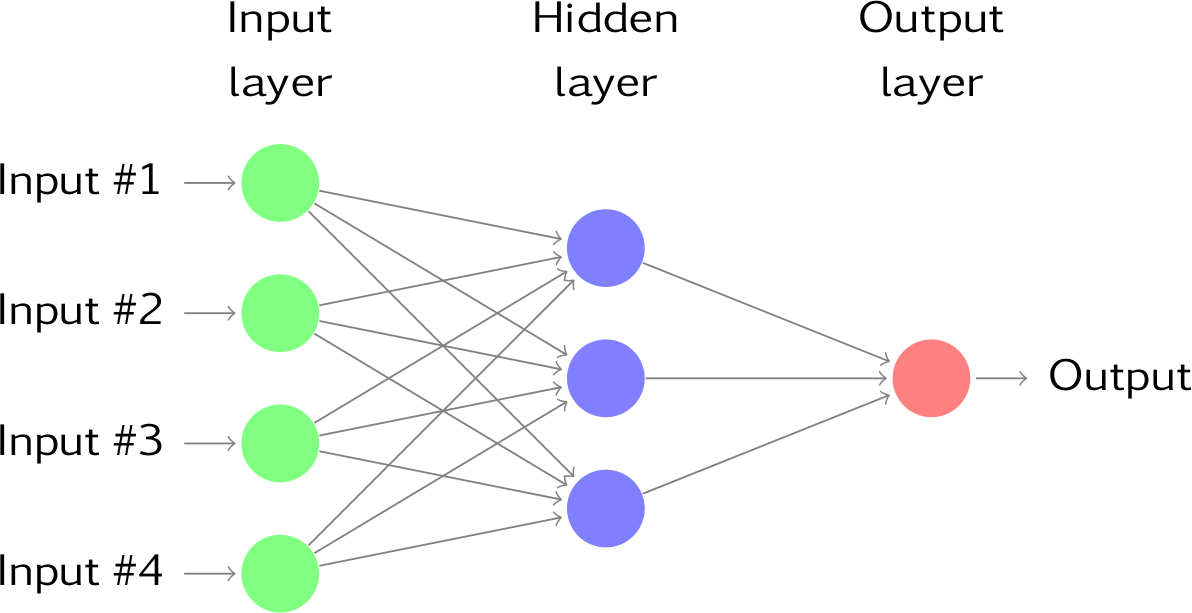
\includegraphics[width=0.6\textwidth]{obrazky-figures/nn_structure.png}
  \caption{Basic structure of a feedforward neural network.
  Source: \cite{hyndman2021forecasting}.}
  \label{fig:nn_structure}
\end{figure}

A feedforward neural network organizes neurons into an input layer, one or more hidden layers, and an output layer, as illustrated in Figure~\ref{fig:nn_structure}. The input layer receives raw data or extracted features; hidden layers transform the input into increasingly abstract representations; and the output layer produces the final prediction. By stacking multiple hidden layers, neural networks can learn hierarchical feature representations, where lower layers capture simple patterns, and higher layers represent more complex structures.

Training a neural network means adjusting its weights and biases to minimize a loss function. Gradients are computed efficiently using the \emph{backpropagation} algorithm, which applies the chain rule to propagate error signals from the output layer back through the network. Parameters are then updated using an optimizer such as Adam, an adaptive variant of gradient descent that maintains per-parameter learning rate estimates based on the running mean and variance of the gradients. Adam is less sensitive to the initial learning rate setting than standard SGD and generally converges faster.

Neural networks with many parameters are prone to overfitting. Several regularization techniques help improve generalization. \emph{L2 weight decay} penalizes large parameter values. \emph{Dropout} randomly sets a fraction of neuron activations to zero during each training step, preventing the network from relying on any single feature and encouraging more distributed representations ~\cite{goodfellow2016dl}. \emph{Batch normalization} normalizes the activations at each layer during training, which stabilizes learning and reduces sensitivity to the choice of learning rate. In addition, early stopping is frequently applied by terminating training when validation performance no longer improves.

Neural networks that contain a large number of hidden layers are referred to as deep learning models. Deep models have achieved high performance in application domains such as image classification, speech recognition, and natural language processing, primarily because they can learn hierarchical feature representations from large datasets without manual feature engineering~\cite{goodfellow2016dl}. On embedded systems, however, deep architectures must be compact enough to fit in limited memory, which motivates the use of the 1D-CNN architecture described below.

\subsubsection{One-Dimensional Convolutional Neural Networks}
A 1D-CNN applies learned filters along the time axis of a sequential signal. Given an input $\mathbf{x} \in \mathbb{R}^{T \times C}$, where $T$ is the number of time steps and $C$ is the number of channels, a convolutional layer with kernel size $k$ and $F$ filters computes:
\begin{equation}
  y_f[t] = \sum_{c=1}^{C} \sum_{\tau=0}^{k-1} w_{f,c}[\tau]\, x_c[t + \tau] + b_f,
\end{equation}
where $w_{f,c}[\tau]$ are the learnable weights and $b_f$ is the bias. Each filter detects a specific local pattern, such as a rapid acceleration peak or a characteristic oscillation. By stacking multiple convolutional layers, the network learns increasingly abstract temporal features, from simple peaks in the first layer to full gesture patterns in later ones. After each convolutional layer, \emph{max pooling} takes the maximum value in each window, keeping the strongest feature activations while making the representation smaller. This reduces computation in later layers and makes the model less sensitive to the exact timing of a gesture within the window.

Once the convolutional stack has extracted compact temporal features, the remaining temporal dimension must be collapsed to a fixed-size vector before classification. \emph{Flatten} does this by concatenating all time steps into one long vector, but its length depends on the input window size. \emph{Global Average Pooling} (GAP) instead computes the mean of each filter's activations across all remaining time steps, producing a vector of size $F$ regardless of window length. GAP results in fewer parameters in the following dense layer and is less sensitive to the exact location within the window where a gesture occurs. A fully connected layer and a softmax output then map this vector to class probabilities.

1D-CNNs are widely used for sensor-based time-series classification because they do not require manual feature engineering, generalize well across recording sessions, and can be deployed efficiently on embedded hardware after quantization~\cite{fawaz2019tsc,warden2018speech}.

\section{Evaluation metrics}
\label{sec:metrics}
Selecting appropriate evaluation metrics is essential for assessing model performance honestly. The most straightforward metric is \textbf{accuracy}, defined as the proportion of correctly classified samples:
\begin{equation}
  \text{Accuracy} = \frac{\text{Number of correct predictions}}{\text{Total number of samples}}.
\end{equation}
While accuracy provides a simple and intuitive performance measure, it may be insufficient for multi-class problems or imbalanced datasets, where a model that always predicts the majority class may achieve high accuracy while failing entirely on the remaining classes.

A more detailed picture is provided by the \textbf{confusion matrix}, which presents the number of predictions for each combination of true and predicted class labels. Each row corresponds to the true class and each column to the predicted class; the diagonal entries are correct predictions, and all off-diagonal entries are errors. The confusion matrix shows not only how often the model is wrong, but which specific classes are confused with each other. An example for a binary problem is shown in Figure~\ref{fig:confusion_example}.


\begin{figure}[H]
  \centering
  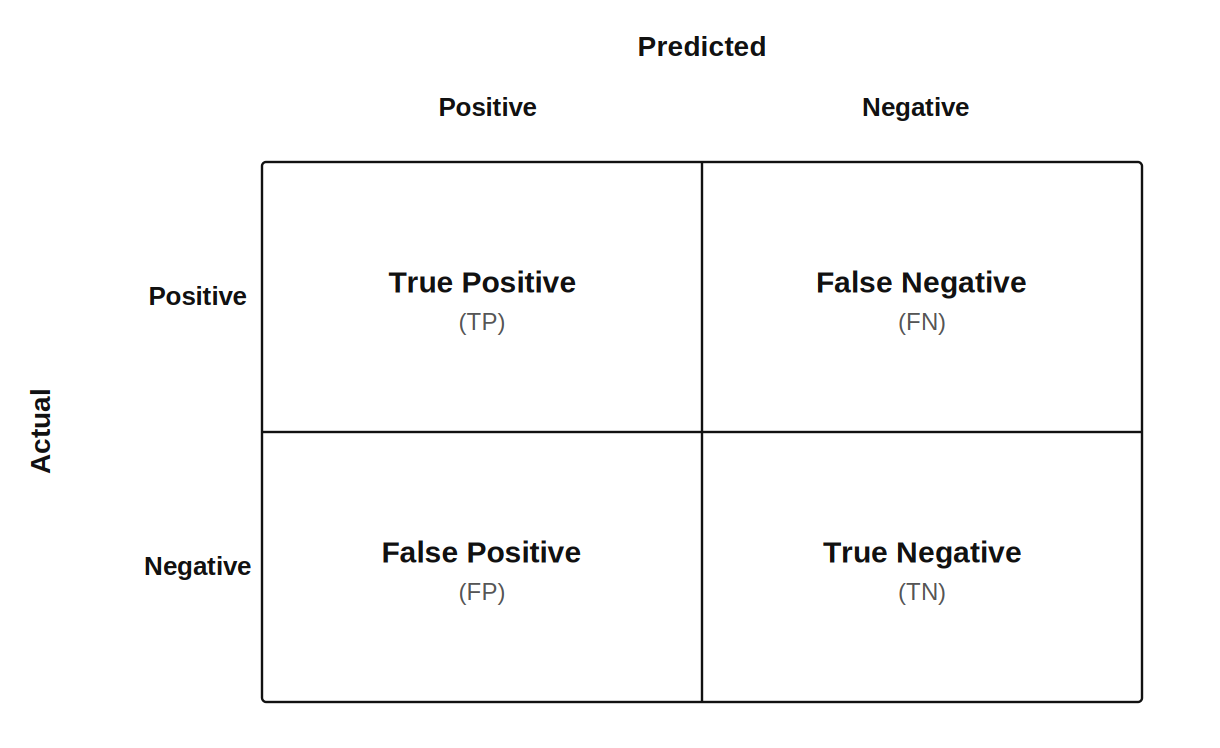
\includegraphics[width=0.8\textwidth]{obrazky-figures/confusion_matrix.png}
  \caption{Structure of a binary confusion matrix. In multi-class problems, the matrix extends to N×N, where N is the number of classes.}
  \label{fig:confusion_example}
\end{figure}

From the confusion matrix, three complementary metrics can be derived.
\textbf{Precision} measures the proportion of positive predictions that are correct:
\begin{equation}
  \text{Precision} = \frac{TP}{TP + FP},
\end{equation}
\textbf{Recall} (also called sensitivity or true positive rate) measures the proportion of actual positive instances that are correctly identified:
\begin{equation}
  \text{Recall} = \frac{TP}{TP + FN},
\end{equation} 
The \textbf{F1-score} combines precision and recall into a single value by taking their harmonic mean:
\begin{equation}
  \text{F1} = 2 \cdot \frac{\text{Precision} \cdot \text{Recall}}{\text{Precision} + \text{Recall}}.
\end{equation}

Since classification models output a probability rather than a hard label, the choice of threshold $\tau$ directly affects which points appear on the ROC curve. The \textbf{Receiver Operating Characteristic} (ROC) curve plots the true positive rate against the false positive rate (FPR) at every possible threshold value:
\begin{equation}
  \text{FPR} = \frac{FP}{FP + TN}.
\end{equation}
Each point on the ROC curve corresponds to a different threshold setting, as illustrated in Figure~\ref{fig:roc_curve}. A model that predicts randomly traces a diagonal line from $(0,0)$ to $(1,1)$, while a perfect classifier reaches the top-left corner $(0,1)$. The \emph{area under the ROC curve} (AUC) summarizes the entire curve as a single number between 0 and 1, where 1 indicates perfect discrimination between classes, and 0.5 corresponds to random prediction. AUC is particularly useful because it evaluates a model across all possible operating points rather than at a single fixed threshold, making it a robust summary metric when the optimal threshold is not known in advance. 

\begin{figure}[H]
  \centering
  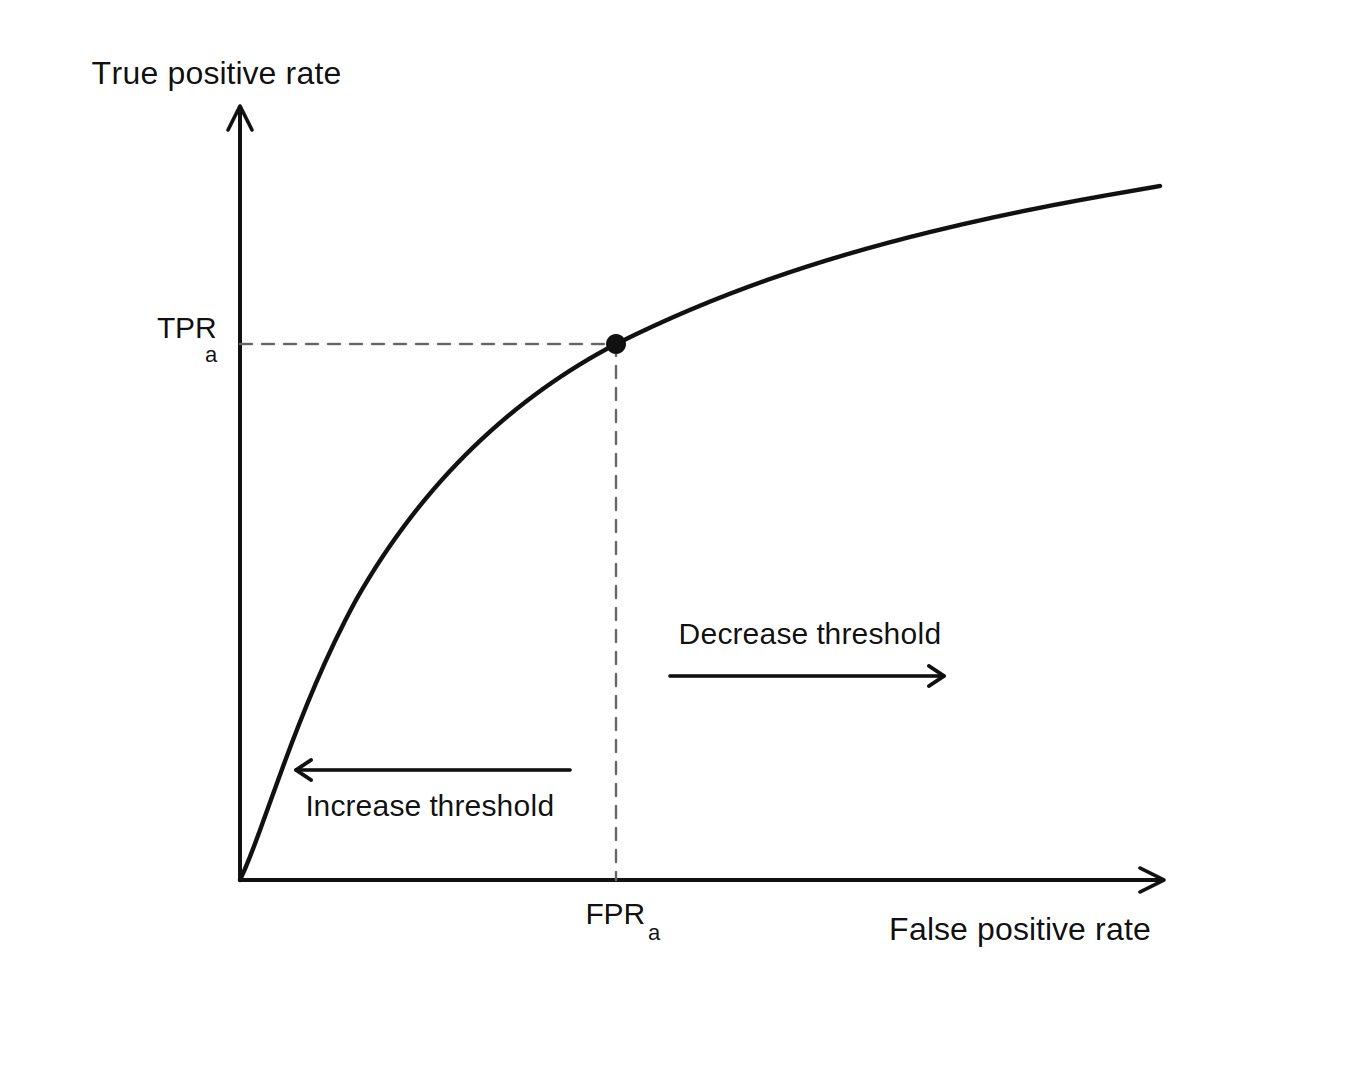
\includegraphics[width=0.8\textwidth]{obrazky-figures/roc_curve.png}
  \caption{Illustration of a ROC curve. Each point on the curve corresponds to a different classification threshold $\tau$. Increasing $\tau$ moves the operating point left; decreasing $\tau$ moves it right. The AUC measures the area under the entire curve.}
  \label{fig:roc_curve}
\end{figure}

In addition to classification performance, embedded machine learning systems need to be evaluated at the system level. \textbf{Inference latency} measures the time needed to produce a prediction from an input sample, directly determining whether real-time operation is feasible. \textbf{Memory footprint} includes both the program memory required to store model weights and the SRAM used for intermediate activations during inference. In some applications, energy consumption is also considered an important evaluation metric, as embedded devices are frequently battery-powered \cite{warden2019tinyml}. 

\section{Common Applications of Machine Learning}

Machine learning is used in many areas, each characterized by specific data types, problem formulations, and evaluation methods. These differences influence both the choice of machine learning models and the datasets used for training and benchmarking.

One of the most common applications of machine learning is image classification, where models are trained to assign semantic labels to visual content. Machine learning techniques in this field are applied to tasks such as object recognition, visual inspection, and understanding scenes. Benchmark datasets such as MNIST, which consists of grayscale images of handwritten numbers \cite{lecun1998mnist}, and CIFAR-10, which contains color images from ten different object categories \cite{krizhevsky2009cifar}, are widely used for evaluating and comparing model architectures.

Speech and audio processing is another important application area, where machine learning techniques are used for tasks such as speech recognition, keyword spotting, and sound event detection. Datasets in this domain typically contain labeled audio recordings, which are often processed as time-series signals or frequency-domain representations. Audio-based applications are particularly relevant to embedded systems because they require continuous, low-latency processing on battery-powered devices. The Speech Commands dataset~\cite{warden2018speech} is a standard benchmark for embedded keyword spotting.

Anomaly detection focuses on identifying patterns in data that differ from normal behavior and is commonly applied in industrial monitoring and fault detection. Machine learning models for anomaly detection are often trained exclusively on normal data, with anomalies flagged as outliers~\cite{chandola2009anomaly}. This paradigm is relevant to embedded systems where the range of possible anomalous events is difficult to define in advance. 

Time-series classification is commonly applied in domains where data are collected as sequences over time. Examples include sensor analytics, healthcare monitoring, finance, and energy systems. Machine learning techniques are used to identify temporal patterns, trends, or repeating structures in sequential data. Time-series datasets are often divided into fixed-length segments and used to evaluate models that operate on streaming or sequential inputs \cite{fawaz2019tsc}.

Sensor-based activity recognition represents a specific and practically important application of time-series classification. In this domain, human activities are recognized using data collected from inertial sensors, such as accelerometers and gyroscopes. Machine learning models typically classify activities such as walking, sitting, or running using extracted temporal features or raw sensor windows. Widely used public datasets include the UCI Human Activity Recognition dataset \cite{anguita2013uci}, the WISDM dataset \cite{kwapisz2011wisdm}, and the PAMAP2 dataset \cite{reiss2012pamap2}. These datasets differ in sensor placement, sampling frequency, number of subjects, and complexity of activities. They are often used to evaluate the performance of activity recognition algorithms. 

The last two categories — time-series classification and sensor-based activity recognition — are the most directly relevant to this thesis, and the datasets introduced here (UCI HAR) are used in Chapter \ref{chap:results}.

\chapter{Embedded Machine Learning}
\label{chap:embedded}

While the previous chapter introduced machine learning from a general theoretical perspective, this chapter focuses on the specific constraints and design principles associated with deploying machine learning models on microcontroller-based embedded systems.

\section{Embedded Machine Learning Context}
% ML on resource-constrained devices
% Differences between cloud ML and embedded ML
% Advantages of embedded ML and constraints

Traditionally, machine learning has been developed and executed on high-performance computing platforms - servers equipped with GPUs, cloud platforms, or, at a minimum, general-purpose laptops. In these environments, both training and inference are performed using powerful hardware with large memory capacity and high computational throughput, and stable power supplies. This allows the use of complex model architectures and large datasets, but it also introduces dependencies on network connectivity, higher energy consumption, and increased system latency.

Embedded machine learning represents a shift from this paradigm by moving inference closer to the data source. Instead of sending raw sensor data to remote servers, an embedded system makes predictions locally in real time. This brings several practical advantages: latency is reduced because no network round-trip is required; data privacy is improved because sensitive information never leaves the device; and the system can continue operating autonomously even when connectivity is unavailable.

The price of these advantages is a set of strict hardware constraints:
\begin{itemize}
    \item limited computational performance,
    \item restricted on-chip memory capacity,
    \item strict energy consumption requirements,
    \item real-time execution constraints.
\end{itemize}

As a result, embedded machine learning systems require adapted model architectures, simplified computations, and careful memory management. Unlike the cloud setting, where accuracy is typically the sole optimization objective, embedded machine learning demands a careful balance between predictive performance, latency, and resource consumption.

\subsection{TinyML as a Specialized Embedded Machine Learning Paradigm}

TinyML is a term used to describe machine learning inference on ultra-low-power microcontrollers, typically those with extremely limited memory and energy availability \cite{warden2019tinyml}. As a result, TinyML solutions rely on compact model architectures, reduced numerical precision, and highly efficient data processing.

It is important to understand that TinyML is not a specific software framework or development tool but rather a design paradigm: it represents the principle of performing meaningful inference directly on deeply embedded hardware, without dependence on cloud connectivity. 

Typical TinyML applications include sensor-based classification, keyword spotting, and anomaly detection. All require continuous, low-latency, energy-efficient operation. The TinyML paradigm is therefore particularly relevant to this thesis, which aims to run gesture classification in real time on an NXP i.MX RT1050 microcontroller.


\section{Classical Machine Learning Models on Microcontrollers}
\label{sec:emb_cl_model}
Chapter~\ref{chap:theory} described the mathematical principles of each model used in this thesis. This section explains how those models are deployed on embedded hardware and the practical constraints.

Logistic regression stores only a weight matrix of size $C \times d$ and a bias of length $C$, where $C$ is the number of classes and $d$ the number of input features. Inference is a single matrix-vector multiply and softmax — constant time, constant memory, independent of training set size.

Linear support vector machines offer similar computational characteristics. Non-linear kernel SVMs, however, require storing all support vectors and computing kernel distances during inference, which typically exceeds microcontroller capabilities.

The $k$-nearest neighbors algorithm does not involve explicit parameter learning, but its inference procedure requires computing distances to every training sample and selecting the $k$ closest ones. Both memory and inference time, therefore, scale with the size of the training dataset. On a microcontroller with limited RAM, storing a training set of several thousand samples is often infeasible, making kNN a poor choice for practical deployment.

Decision trees are particularly attractive for embedded deployment due to their rule-based structure. During inference, a decision tree evaluates a sequence of simple conditional statements, which can be efficiently implemented using if--else logic in low-level programming languages. The memory footprint is proportional to the number of nodes, which can be controlled by limiting tree depth. Shallow trees are efficient but may underfit; deeper trees improve accuracy but consume more memory and may generalize poorly.
Random forests improve generalization substantially but multiply the memory requirement by the number of trees.

\section{Neural Networks on Embedded Systems}
% Discusses lightweight neural networks for embedded platforms.
% Explains limitations of deep learning on microcontrollers.
The most important architectural principle for deployment of embedded neural networks is the separation of training and inference. Training is performed offline on desktop or server hardware. Only the trained model parameters are transferred to the embedded device, which only performs the forward pass during deployment. This means the embedded system never computes gradients, stores optimizer state, or processes the full training dataset, which significantly reduces the required resources.

Even so, neural network models must be designed with the target platform in mind. Memory constraints manifest in two distinct ways. The model weights and biases must be stored in flash memory, which is non-volatile but limited. During inference, intermediate activations must be held in SRAM, which is faster but even more constrained. A model with a small parameter count can still fail to fit in memory if its intermediate activations are large, as in the case with wide convolutional layers applied to long input sequences.

Inference latency is an equally important constraint. Embedded applications such as gesture recognition typically require predictions within tens of milliseconds to feel responsive to the user. A model that achieves excellent accuracy but requires several seconds per inference is not practically deployable. Measuring and reporting latency is therefore an essential part of embedded model evaluation, alongside accuracy and memory footprint.

The 1D-CNN architecture in this thesis was designed with both constraints in mind: moderate filter counts, small kernel sizes, and a single pooling layer keep the activation memory budget manageable while achieving competitive accuracy. Measured inference latency and memory footprint for all model variants are reported in Chapter~\ref{chap:results}.

\section{Model Optimization for Embedded Systems}
Even a carefully designed compact model may need further optimization before it can be deployed on a microcontroller. The primary goal of post-training optimization is to reduce memory and computational requirements while preserving as much predictive accuracy as possible.

\subsection{Quantization}
Quantization is one of the most widely used optimization techniques in embedded machine learning. Its principle is to represent model weights and activations using lower-precision numerical formats rather than the 32-bit floating-point values used during training \cite{jacob2017quantization}. The most common target is 8-bit integer (int8) quantization, which reduces model size and allows inference to use integer arithmetic, which is faster and more energy-efficient on processors without dedicated floating-point units.

The quantization process maps floating-point values $r$ to integer values $q$ through a linear transformation:
\begin{equation}
  q = \text{round}\!\left(\frac{r}{S}\right) + Z,
\end{equation}
where $S$ is a scale factor and $Z$ is a zero-point offset, both determined by the range of values observed in the floating-point model. The inverse transformation recovers an approximation of the original value:
\begin{equation}
  \hat{r} = S \cdot (q - Z).
\end{equation}
This approximation introduces a small quantization error, which can reduce classification accuracy. In practice, the accuracy loss from int8 quantization is typically minor — often less than one percentage point — and is an acceptable tradeoff for the gains in model size and inference speed~\cite{warden2018speech}.

TensorFlow Lite supports two quantization modes evaluated in this thesis. \textbf{Dynamic range quantization} quantizes only the model weights to int8 at conversion time, while activations remain in float32 during inference. This mode requires no representative calibration data and is straightforward to apply, but inference speed gains are more limited. \textbf{Full integer quantization} (int8) quantizes both weights and activations, requiring a small representative dataset for calibration to determine the activation ranges. This mode achieves the maximum reduction in both model size and inference latency and is the recommended approach for microcontroller deployment. The measured outcomes for both modes on the baseline gesture
model are reported in Table~\ref{tab:quantization}.

\subsection{Pruning and Structural Simplification}
Model pruning is an optimization technique that reduces the size and computational complexity of models by removing parameters with limited impact on the model's output. One common pruning strategy is weight pruning, which removes individual connections with small absolute values after training \cite{han2015pruning}. After pruning, the model is typically fine-tuned to recover any lost accuracy.

Structural pruning removes entire neurons, convolutional filters, or layers, producing a smaller dense model with predictable reductions in memory and computation. This is often more practical for embedded deployment than weight pruning. In this thesis, structural simplification is achieved by varying the number of convolutional filters across experiments, which directly controls both the model's capacity and its memory footprint. 

\subsection{Other Efficiency Methods}

In addition to quantization and pruning, a number of additional techniques can be used to improve the performance of machine learning models. For example, input data preprocessing and feature selection can significantly reduce computational load by limiting the amount of data processed during inference. By extracting only the most relevant features, the model complexity can be reduced without modifying the model itself.

Another common method is knowledge distillation in which a small model is trained to repeat the behavior of a larger, more accurate model, called a teacher. While the teacher model may be too complex to deploy on an embedded device, a student model can achieve competitive results while requiring significantly fewer resources \cite{hinton2015distillation}. 

Additional efficiency gains can be obtained through operation fusion, which combines sequential operations such as convolution, batch normalization, and activation into a single computational step, reducing memory access overhead. TensorFlow Lite applies several such fusions automatically during model conversion.

\chapter{Related Work}
\label{chap:related_work}

Deploying machine learning on a microcontroller means working within hard limits that do not exist on a laptop or a server: memory is measured in kilobytes, the processor has no GPU, and the power budget is often in the milliwatt range. These constraints are not just inconvenient --- they determine which models can even be considered and what must be measured to call a system deployable. Batzolis et al.~\cite{batzolis2023ml} survey embedded machine learning systems and identify memory, inference latency, and energy as the three constraints that shape most design decisions in the field. They also note that many papers report only accuracy, making practical comparisons difficult. Banbury et al.~\cite{banbury2021mlperftiny} address this directly with MLPerf Tiny, a benchmark suite that standardizes four embedded tasks and requires measuring latency and binary size alongside accuracy. The need for a shared protocol like this reflects how young and fragmented the field is. Warden and Situnayake~\cite{warden2019tinyml} offer the most widely used practical guide to building within these constraints, covering the full path from training to on-device deployment with integer quantization. 

Sensor-based gesture recognition is one of the tasks that fits naturally into this setting, as it requires continuous, low-latency inference directly on the device, with no network connection and no cloud processing, which makes the constraints described above unavoidable. Before deep learning became practical on microcontrollers, gesture recognition was usually done with hand-crafted similarity measures and template matching. Ji et al.~\cite{ji2015gesture} use a single 3-axis accelerometer with a fast variant of dynamic time warping (FastDTW) and a two-scaled normalization step that compensates for amplitude differences between repetitions of the same gesture. They report 99\% accuracy on 16 gesture classes with only five training samples per class, and FastDTW is about eight times faster than standard DTW on the same data. The method needs almost no training and runs on very modest hardware, but the recognition logic has to be redesigned for every new gesture set, and accuracy is known to drop as the number of classes increases.

More recent work moves away from hand-crafted templates and applies small neural networks directly to the raw signal. The review by Ismail Fawaz et al.~\cite{fawaz2019tsc} compares nine deep architectures across the UCR/UEA time-series archive and finds that 1D convolutional networks tend to match or outperform recurrent models while being faster to train and more predictable in their memory use --- a property that matters a lot when the target is a device with a few hundred kilobytes of SRAM, since recurrent models must keep a hidden state across time steps whose size is hard to estimate in advance. Two recent papers follow this approach all the way to deployment on a microcontroller and are directly relevant to the work in this thesis. Saha et al.~\cite{saha2024wrist} build a TinyML system for wrist-worn IMU gesture recognition: a small 1D-CNN is trained, quantized to 8-bit integers using TensorFlow Lite, and deployed on a microcontroller, reaching around 97\% accuracy with the model size and on-device memory footprint reported. The pipeline is close to the one used in this thesis, but only a single neural model is evaluated, and no classical baselines are included, so it is hard to judge whether the chosen architecture was actually necessary for the task. Grabarczyk and Lazarowska~\cite{grabarczyk2025} take a broader approach: they train and compare three model families --- a multi-layer perceptron, a support vector machine, and a random forest --- on a microcontroller-based gesture recognition system aimed at drone control and assistive applications, and evaluate them using F1-scores on the target hardware. Their main finding is that the random forest is the most efficient model for their task. This is the closest existing work to the comparison carried out in this thesis, though on-board latency and memory are not reported in detail alongside the accuracy metrics. Together, these two papers show that both neural and classical models can be made to work for IMU gesture recognition on a microcontroller; what remains less explored is how they behave when all system-level metrics --- accuracy, memory, and on-board latency --- are measured and reported side by side for the same task on the same hardware.

A question that the gesture recognition literature leaves open is when a neural network is actually needed over a classical model. The answer depends mostly on how much training data is available. Fern\'andez-Delgado et al.~\cite{fernandez2014classifiers} compared 179 classifiers across 121 datasets and found that random forests and well-tuned linear models are difficult to outperform when data is limited. Sanchez-Iborra and Skarmeta~\cite{sanchez2020tinyml} make the same observation from the TinyML angle: on small sensor problems, a classical model often matches a small neural network while using much less memory, and its inference can be implemented directly in C without any runtime at all. The UCI Human Activity Recognition benchmark by Anguita et al.~\cite{anguita2013uci} represents the larger-data end of this spectrum, with 21 training subjects and 9 test subjects across six activity classes. It is the standard reference for sensor-based activity recognition, and published results on it --- around 96\% with an SVM on hand-crafted features in the original paper and around 95\% with a 1D-CNN on raw signals by Ronao and Cho~\cite{ronao2016deep} --- give a useful baseline for what a reasonable model should achieve on a large, diverse dataset. On a much smaller dataset, such as the two-subject gesture corpus collected for this thesis, the literature suggests the picture may look quite different, and exploring that difference is part of what the experimental chapters report.

\chapter{Embedded Platforms and Software Ecosystem for Machine Learning}
\label{chap:platforms}

\section{Overview of Embedded and Edge Platforms}
% Microcontrollers: STM32, ESP32, NXP i.MX RT series
% Single-board computers: Raspberry Pi
Embedded and edge machine learning can be deployed on various hardware platforms ranging from ultra-low-power microcontrollers consuming microwatts to powerful edge AI accelerators capable of running large neural networks in real time.

\paragraph{Microcontroller-based platforms}

Microcontrollers are the most resource-constrained class of embedded ML hardware. They combine a processor core, on-chip memory, and peripheral interfaces into a single chip and are designed for deterministic real-time behavior at low power. Despite these limitations, recent advances in hardware design and optimized software libraries have enabled the use of machine learning on microcontrollers for tasks such as sensor-based classification, anomaly detection, and control applications. 
Common microcontroller families used in embedded ML include the ESP32 and STM32 families. These are widely used because of their low power consumption, rich peripheral integration, and large ecosystem support~\cite{esp32,stm32}. Efficient neural network execution on ARM Cortex-M devices is supported by CMSIS-NN\cite{cmsisnn}.

\paragraph{High-performance embedded platforms}

Between basic microcontrollers and single-board computers sits a class of high-performance embedded platforms, sometimes called crossover or hybrid systems. These combine the real-time determinism of a microcontroller with significantly higher computational performance and memory capacity.

The NXP i.MX RT series is a representative example. It uses high-frequency ARM Cortex-M cores together with advanced memory subsystems, enabling more demanding machine learning tasks while maintaining deterministic real-time behavior~\cite{nxpimxrt}. The Arduino Portenta H7 is another example, designed for high-performance embedded applications with increased compute and memory resources compared to standard microcontrollers~\cite{portentah7}. These platforms are used when a basic microcontroller is not powerful enough, but the overhead of a full operating system is undesirable.

\paragraph{Single-board computers}

Single-board computers represent the upper end of the embedded computing spectrum. They run a full operating system, most commonly Linux, and provide enough processing power and memory to use standard machine learning frameworks without significant modification. The Raspberry Pi family is widely used in edge computing, rapid prototyping, and educational settings~\cite{raspberrypi}. The higher performance comes at the cost of more power consumption and weaker real-time guarantees compared to microcontroller-based solutions.

\paragraph{Specialized machine learning accelerators}

Dedicated hardware accelerators have been developed to meet the growing compute demands of edge machine learning. These devices speed up neural network inference by performing matrix operations on dedicated hardware units. The Google Edge TPU is a common example, often used together with single-board computers or embedded Linux systems~\cite{edgetpu}. Such accelerators can significantly improve inference throughput and energy efficiency, but they are typically limited to specific frameworks and model architectures, which reduces portability.

Table~\ref{tab:platform_comparison} summarises the key properties of representative platforms across these categories.

\begin{table}[ht]
  \centering
  \caption{Comparison of representative embedded and edge ML platforms.}
  \label{tab:platform_comparison}
  \small
  \begin{tabular}{p{3.0cm}p{2.4cm}p{1.5cm}p{1.6cm}p{1.5cm}p{2.8cm}}
    \toprule
    \textbf{Platform} & \textbf{Processor} & \textbf{Clock} &
    \textbf{SRAM} & \textbf{Flash} & \textbf{Category} \\
    \midrule
    Arduino Nano 33 BLE & Cortex-M4    & 64\,MHz  & 256\,KB  & 1\,MB  & Ultra-low-power MCU \\
    ESP32               & Xtensa LX6   & 240\,MHz & 520\,KB  & 4\,MB+ & Standard MCU \\
    STM32H7             & Cortex-M7    & 480\,MHz & 1\,MB    & 2\,MB  & High-perf.\ MCU (single-core)\\
    \textbf{NXP i.MX RT1050} & \textbf{Cortex-M7} & \textbf{600\,MHz} &
      \textbf{512\,KB} & \textbf{2\,MB} & \textbf{Crossover MCU} \\
    Arduino Portenta H7 & Cortex-M7+M4    & 480/240 \,MHz & 1\,MB    & 2\,MB  & High-perf.\ module (STM32H747) \\
    Raspberry Pi 4      & Cortex-A72   & 1.8\,GHz & 4\,GB    & SD     & Single-board PC \\
    \bottomrule
  \end{tabular}
\end{table}


\section{Software Ecosystem for Embedded Machine Learning}
% General ML Frameworks: Keras, PyTorch
% Embedded ML Libraries and Toolchains: TensorFlow Lite, TensorFlow Lite Micro, Edge Impulse
% Vendor-specific tools: NXP eIQ, STM NanoEdge AI Studio
\subsection{Model Training Frameworks}

Model training is typically performed on general-purpose hardware using high-level machine learning frameworks that provide automatic differentiation, efficient numerical computation, and a broad range of pre-built model components.

\textbf{Keras} is a high-level API for neural networks, now integrated as the standard interface for TensorFlow. It enables rapid prototyping through a readable, layer-oriented programming model and supports the full range of architectures used in this thesis, including convolutional and fully connected networks \cite{tensorflowkeras}. 

\textbf{PyTorch} is an alternative framework emphasizing flexibility and dynamic computation graphs. This design allows developers to modify model behavior during runtime,  which simplifies the implementation of non-standard architectures and training procedures \cite{paszke2019pytorch}. While PyTorch is widely used in research, it was not used in this thesis; trained models would need to be exported to ONNX format and then converted to a microcontroller-compatible representation.

\subsection{LiteRT (TensorFlow Lite)}

TensorFlow Lite, recently rebranded as LiteRT, is the primary framework for deploying neural network models on mobile and embedded devices~\cite{litert}. It provides a complete pipeline from trained model to on-device inference, covering model conversion, optimization, and a lightweight runtime suitable for microcontrollers.

The conversion process takes a trained Keras or TensorFlow model and produces a FlatBuffer binary file with the \texttt{.tflite} extension. During conversion, TensorFlow Lite applies automatic optimizations, including operator fusion and dead code elimination.

Quantization is applied at conversion time using the \texttt{TFLiteConverter} API. For dynamic range quantization, no additional data is required; for full int8 quantization, a small representative dataset.

\textbf{TensorFlow Lite for Microcontrollers} (TFLite Micro) is a specialized port of the TFLite runtime designed for devices without operating systems, dynamic memory allocation, or file systems. It is implemented as a pure C++ library with no external dependencies, making it portable across ARM Cortex-M and other embedded architectures. TFLite Micro supports a set of operations sufficient for most CNN, MLP, and RNN inference tasks, and integrates with CMSIS-NN for hardware-accelerated execution on ARM processors.

\subsection{CMSIS-NN}

CMSIS-NN is a collection of highly optimized neural network kernel functions developed by Arm for Cortex-M processors~\cite{cmsisnn}. Unlike complete inference frameworks, CMSIS-NN operates at a low abstraction level, it provides hand-optimized implementations of convolution, depthwise convolution, fully connected layers, and activation functions that use the SIMD (Single Instruction, Multiple Data) capabilities of the ARMv7-M and ARMv8-M instruction sets. By processing multiple data elements in a single instruction, CMSIS-NN can reduce inference latency and power consumption compared to generic C implementations. 
In practice, CMSIS-NN is used as a backend by TFLite Micro rather than directly. TFLite Micro dispatches operations to CMSIS-NN automatically when it detects a supported Cortex-M target.

\subsection{Edge Impulse}
Edge Impulse is a cloud-based development platform that integrates data collection, signal processing, feature extraction, model training, and deployment into a single workflow. It supports both classical machine learning models and compact neural networks, and produces optimized C++ inference code targeting a wide range of embedded platforms~\cite{edgeimpulse}. The key advantage of Edge Impulse is its rapid prototyping capabilities and powerful visualization tools that help developers understand sensor data and model behavior. However, the high level of abstraction limits low-level customization. Advanced control over memory layout, operator implementation, or numerical precision is limited compared to manual toolchains.

\subsection{NXP eIQ}
The NXP eIQ is a software development environment developed by NXP Semiconductors. It is designed to support the deployment of machine learning on NXP microcontrollers and processors, including the i.MX RT series used in this thesis. The eIQ toolkit combines various inference engines, such as TensorFlow Lite Micro and CMSIS-NN, and provides tools for model transformation, optimization, and performance profiling. It also supports hardware acceleration capabilities present on specific NXP platforms. This close integration enables developers to efficiently map machine learning workloads to NXP hardware. Also, one of the key features of NXP eIQ is its support for automated model generation and optimization using AutoML techniques. Through integrated tools such as eIQ AutoML and eIQ Toolkit, the framework can automatically explore different model architectures, feature representations, and hyperparameter configurations to identify solutions that best fit the constraints of the target embedded platform. However, the main limitation of eIQ is its platform-specific nature, which limits its portability to non-NXP devices\cite{nxpeiq}.

\subsection{STM NanoEdge AI Studio}
NanoEdge AI Studio, developed by STMicroelectronics, is an AutoML tool that automatically explores signal processing pipelines, feature extraction methods, and machine learning model configurations to find solutions optimized for a specific STM32 target device~\cite{nanoedge}. The resulting model is exported as a compact standalone C library for direct integration into STM32 firmware. 
NanoEdge AI Studio is primarily designed for rapid prototyping and industrial applications, where reliability and development speed are more important than full control over the model's internal mechanisms. While the tool significantly simplifies the deployment of embedded machine learning, it offers limited insight into the internal structure of the model and the optimization methods used.

\section{Monitoring, Debugging, and Profiling}
Unlike traditional machine learning environments, where diagnostic and monitoring tools are easily available, embedded systems operate under strict hardware constraints and limited runtime visibility. As a result, monitoring, debugging, and profiling become necessary to verify the correctness of model behavior and ensure that machine learning applications meet real-time and resource requirements.

\emph{Training monitoring} is performed during the offline training phase on desktop hardware. Tools such as TensorBoard are commonly used to provide visualization of training and validation loss curves, accuracy trends, and other metrics over epochs, which helps identify overfitting, learning rate issues, and convergence problems before deployment \cite{tensorboard}.

After deploying a trained model to an embedded platform, monitoring focuses on runtime behavior and data flow. This includes verifying the correctness of sensor inputs, model output, and interactions with surrounding application logic. In embedded systems, monitoring is often implemented using lightweight logging mechanisms, serial output, or hardware indicators (for example LEDs). 

\emph{Debugging} addresses functional errors and integration issues that can arise when combining machine learning models with embedded software. Embedded debugging is typically performed using integrated development environments (IDEs) such as the MCUXpresso IDE \cite{mcuxpressoide}, which provide support for breakpoints, memory inspection, and step-by-step execution. On systems using a real-time operating system (RTOS), additional information can be obtained using FreeRTOS tracing, which enables analysis of task scheduling, execution time, and system load \cite{freertostrace}. These debugging capabilities are important for identifying timing issues and resource contention that arise during inference.

\emph{Profiling} focuses on measuring system performance and resource usage. In the context of embedded machine learning, profiling typically includes measuring inference latency, memory consumption, and, in some cases, power consumption. Profiling in embedded systems often requires explicit instrumentation, such as measuring execution times using hardware timers or analyzing the sizes of compiled binaries \cite{warden2019tinyml}. These measurements provide concrete evidence of system performance and allow for objective comparisons of different models and deployment configurations. Profiling results are typically used to identify optimization strategies and evaluate tradeoffs between model accuracy, latency, and memory usage.

Together, monitoring, debugging, and profiling form a critical feedback loop in embedded machine learning development. The methods discussed in this section are applied in the experimental part of this thesis to evaluate the deployed machine learning models.

\chapter{Experimental Design and Implementation}
\label{chap:design}

This chapter describes the complete pipeline from physical hardware setup to trained and deployed model. It covers the hardware configuration, data collection procedure, dataset organization, preprocessing and feature extraction, model architecture and training, TFLite export and quantization, and the firmware that runs live inference on the target board.

\section{Experimental Overview}
% High-level overview of the implemented solution.
The experimental work in this thesis consists of two complementary studies.
 
The first uses the publicly available UCI Human Activity Recognition dataset~\cite{anguita2013uci} as an implementation validation benchmark. Before collecting custom sensor data and committing to a particular model architecture, it was necessary to verify that the Keras training pipeline, the chosen 1D-CNN architecture, and the TFLite export and quantization workflow all behave correctly on a well-understood problem with a known, reproducible baseline. The UCI dataset is ideal for this purpose: it provides a fixed cross-subject train/test split, a large and diverse subject pool, and has been used extensively in the embedded activity recognition literature, making it possible to detect implementation errors that would be invisible on a small self-collected dataset. As a secondary benefit, the UCI experiments allow a systematic study of hyperparameter sensitivity, because the larger number of training subjects provides more stable results — something that is impossible with only two subjects. The UCI experiments do not involve embedded deployment; all training and evaluation are performed on desktop hardware.
 
The second study covers the full embedded deployment cycle for a custom five-class wrist gesture recognition task. Data was collected from two subjects using a wrist-mounted inertial sensor, both a 1D-CNN and classical machine learning models were trained and evaluated, and the best-performing models were deployed on the NXP i.MX RT1050 evaluation board for real-time inference and live evaluation. This study is the central hardware contribution of the thesis.

The overall pipeline for both studies is shown in Figure~\ref{fig:pipeline_overview}.
 
\begin{figure}[ht]
  \centering
  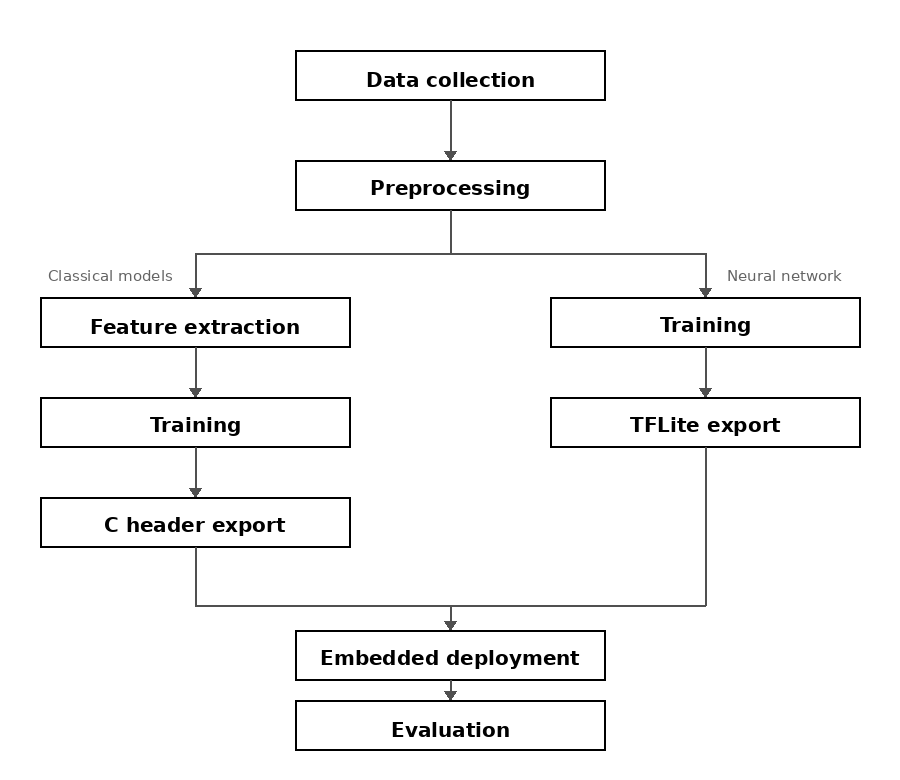
\includegraphics[width=0.78\textwidth]{obrazky-figures/pipeline_workflow.png}
  \caption{Overview of the experimental pipeline. The left branch shows the classical model path; the right branch shows the neural network path.}
  \label{fig:pipeline_overview}
\end{figure}

\section{Hardware Setup}
\label{sec:hardware}

The target platform is the NXP MIMXRT1050-EVK evaluation board. Its processor is an ARM Cortex-M7 running at up to 600\,MHz. The board provides 512\,KB of on-chip SRAM and 2\,MB of flash, with access to an external 64\,MB HyperFlash device for storing larger firmware images and data. A microSD card slot is available on the board and was used for data storage during the collection phase. The Cortex-M7 core includes a floating-point unit and DSP extensions, which accelerate the preprocessing and inference computations. 

The NXP i.MX RT1050 was selected because its Cortex-M7 core represents a mid-range microcontroller with enough resources to run a quantized 1D-CNN comfortably, while the 512\,KB SRAM and 2\,MB flash budget remains tight enough to make the memory optimization experiments meaningful.

The sensor used in the thesis is an InvenSense MPU6050, a six-axis device combining a three-axis accelerometer and a three-axis gyroscope in a single package, communicating with the board over LPI2C1 bus at 400\,kHz. The accelerometer was configured with a full-scale range of $\pm$8\,g and the gyroscope with $\pm$500\,\textdegree/s. These ranges are wide enough to capture fast wrist gestures without saturation, while avoiding the unnecessary quantization noise that would arise from a wider range. A digital low-pass filter with a 42\,Hz cutoff was enabled in hardware to suppress high-frequency noise before sampling. The output data rate was set to 50\,Hz for all recordings and all inference experiments. AD0 is tied to ground, fixing the device address at 0x68. The complete pin mapping is given in Table~\ref{tab:wiring}.

Initially, a prototype was developed using the board's built-in accelerometer to gain familiarity with the embedded data collection pipeline and to build a first simple model. The MPU-6050 was subsequently chosen for the main experiments because a wrist-mounted external sensor captures gesture motion directly at the wrist, which is more appropriate for gesture recognition than a sensor fixed to the evaluation board.

\begin{table}[ht]
  \centering
  \caption{MPU-6050 to MIMXRT1050-EVKB wiring.}
  \label{tab:wiring}
  \begin{tabular}{lll}
    \toprule
    \textbf{MPU-6050 pin} & \textbf{EVKB pin} & \textbf{Description} \\
    \midrule
    VCC & 3.3\,V rail & Power \\
    GND & GND         & Ground \\
    SDA & J23-5 (I2C1\_SDA) & I2C data \\
    SCL & J23-6 (I2C1\_SCL) & I2C clock \\
    AD0 & GND & I2C address = 0x68 \\
    INT & J22-8 & Data-ready \\
    \bottomrule
  \end{tabular}
\end{table}

Development and debugging were done using the MCUXpresso IDE~\cite{mcuxpressoide}, which connects to the board via a built-in JTAG/SWD interface. UART output was used throughout as a lightweight monitoring channel, printing status messages and inference statistics to a connected PC terminal without interrupting the real-time task scheduling.

\section{Data Collection}
% Explains how experimental data were recorded.
 
Five gesture classes were defined for the recognition task, chosen to be practically useful for a simple interactive control interface while remaining physically distinct enough to be reliably separable. The first one, \emph{idle}, includes transitions between gestures, pauses during normal use, and low-amplitude background hand motion. The four active classes are \emph{accept} (a tick shape drawn in the air) \emph{left} (a horizontal swipe to the left), \emph{right} (a horizontal swipe to the right), and \emph{cancel} (a short lateral wrist shake). 

Data was collected by two subjects (Subject~A and Subject~B). Each subject performed five independent recording sessions per class. Sessions were intentionally conducted on different days and different times of day, including morning and evening recordings, to introduce natural variability in gesture amplitude, speed, and wrist position. Each session contained multiple repetitions of the target gesture. The sensor was mounted on a standard watch strap and worn on the wrist of the dominant hand.
 
Each session is stored as a CSV file with columns \texttt{timestamp\_ms}, \texttt{ax\_g}, \texttt{ay\_g}, \texttt{az\_g}, \texttt{gx\_dps}, \texttt{gy\_dps}, \texttt{gz\_dps} at 50\,Hz. Each file was named according to the convention \texttt{<label>\_<subject><session>.csv}, encoding subject identity, gesture class, and session number directly in the filename.

\subsection{Data Validation with Edge Impulse}
\label{sec:edge_impulse}
 
Before implementing the full custom training pipeline, the collected dataset was validated using Edge Impulse~\cite{edgeimpulse} to confirm that the five gesture classes were separable and that the recording procedure had produced a consistent, correctly labeled signal. A prototype model was trained directly within Edge Impulse, targeting the NXP~i.MX~RT1050, allowing both the data quality and the on-device feasibility to be assessed before committing to the custom TFLite Micro workflow.
 
Figure~\ref{fig:ei_features} shows the feature explorer output. The gesture classes mostly form a shared central cluster with some partial grouping, indicating that the features capture common patterns while still preserving some class differences. There is noticeable overlap between similar gestures, such as swipe left, swipe right, and cancel, which may lead to some confusion in the final results.
 
\begin{figure}[ht]
  \centering
  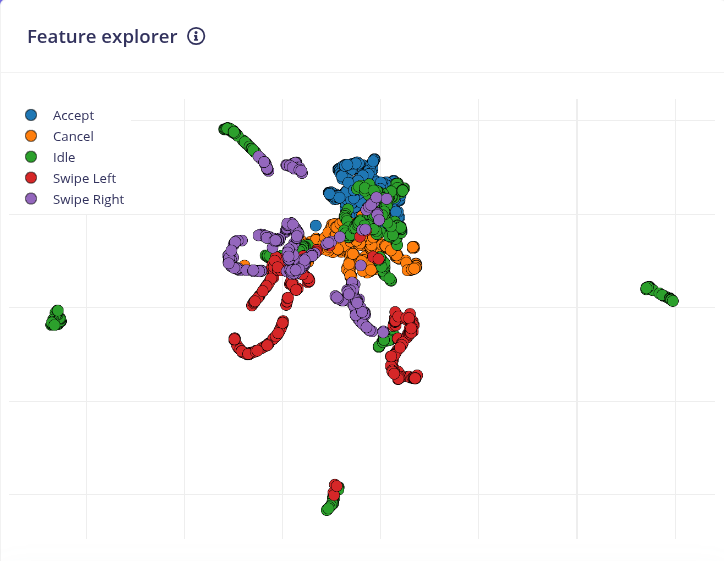
\includegraphics[width=\textwidth]{obrazky-figures/edge_impulse_features.png}
  \caption{Edge Impulse feature explorer for the five gesture classes.}
  \label{fig:ei_features}
\end{figure}

\section{Dataset Organization and Splitting Strategy}
\label{sec:splitting}

The way the data is split is very important in time-series classification, because it affects how reliable the results are. If the split is not done correctly, the reported accuracy can be too high due to similarities between nearby time windows. Therefore, it is important to make sure that data from the same recording session is not used in both training and evaluation.

For the neural network experiments on the custom dataset, each subject has five recording sessions per class. Four sessions are used for training and validation, and one session is used only for testing. This ensures that the model is evaluated on data it has not seen before. A random split at the window level is not suitable because windows from the same recording are very similar and could appear in both training and test sets.

For the classical models, five-fold group cross-validation is used. All windows from the same recording session are kept in the same fold. This keeps the separation between sessions in all evaluation steps. In each fold, the feature scaler is fitted only on the training data and then applied to the test data, so no information from the test set is used during training.

For the UCI HAR dataset, the original split is used, where data from 21 subjects are used for training and 9 for testing. From the training subjects, 20\% are selected as a validation set. This allows model tuning on data that are not used for training.

\section{Signal Preprocessing}
\label{sec:preprocessing}

Raw sensor recordings require three preprocessing steps before they can be used as model input: segmentation into fixed-length windows, per-channel normalization, and optional data augmentation for the neural network pipeline.

\subsection{Signal Segmentation}
 
Both datasets were segmented into fixed-length windows before model training. A window of $W$ samples is extracted starting at position $t$, and the next window starts at $t + S$, where $S$ is the stride. When $S < W$, the windows overlap, which increases the number of training samples and ensures that gesture transitions near window boundaries appear in at least one window.
 
Since each recording session contains a single gesture class repeated throughout, every sample in the session carries the same label. The window label is therefore assigned as the label of the final sample in the window. Each window is represented as a two-dimensional array of shape $(\text{window\_size},\, 6)$, where the six columns correspond to the IMU channels.
 
\subsection{Normalization}
Raw sensor values differ significantly in scale. Without normalization, channels with larger magnitudes, such as those from the gyroscope, would dominate the gradient during training. This can lead to unstable optimization and reduce the model’s ability to learn effectively.

To address this, Z-score normalization is applied independently to each channel. The mean and standard deviation are computed from all time steps across the training windows, resulting in a set of per-channel constants. These parameters are then applied consistently to the training, validation, test, and runtime data.

\subsection{Data Augmentation}
 
To reduce overfitting on the small two-subject dataset, data augmentation was applied during neural network training. When enabled, two random transformations were applied to each training window before it was fed to the model. First, Gaussian noise with a standard deviation of 0.03 (applied after per-window normalization) was added to simulate sensor noise. Second, the entire window was multiplied by an amplitude scale factor sampled uniformly from $[0.92,\,1.08]$ to simulate natural differences in gesture intensity between repetitions and subjects. Augmentation was applied only to training windows; validation and test windows were used unmodified.

\section{Feature Engineering for Classical Models}
\label{sec:features}
 
Classical models require a fixed-length feature vector rather than a two-dimensional time-series array. For each of the six sensor channels, five statistical features were computed per window. The mean value characterizes the average sensor displacement from rest during a gesture, which varies significantly between a motionless hand and a directed hand movement. The mean absolute deviation (MAD) measures the spread of values around the mean value, without being distorted by individual outliers, as can occur with variance. The minimum and maximum values reflect the extremes of the movement trajectory, which are particularly informative for gestures that produce sharp acceleration peaks in one direction. The zero-crossing rate (ZCR) of a signal centered around the mean value counts the number of sign changes within a window, providing a frequency descriptor of the vibrational content without the need for a full spectral transform.
The ZCR counts sign changes in the mean-centered signal:
\begin{equation}
  \text{ZCR} = \sum_{t=1}^{W-1}
    \mathbf{1}\!\left[(x_t - \bar{x})(x_{t+1} - \bar{x}) < 0\right].
\end{equation}
This gives a 30-dimensional feature vector per window ($6 \times 5$). The features were standardized with a \texttt{StandardScaler} fitted on the training partition before being passed to the classifiers. 

\section{Classical Model Training and Embedded Deployment}
\label{sec:classical_training}

\subsection{Classifiers and Training}

Five classical classifiers are trained and evaluated on the 30-dimensional feature vectors: logistic regression, a linear support vector machine (SVM), a decision tree, $k$-nearest neighbors, and a random forest. The classifiers are implemented using scikit-learn with standard default hyperparameters, with the exception of the decision tree, which is limited to a maximum depth of 10 in the UCI experiments to prevent it from growing unbounded on the larger dataset.

In both cross-validation and hold-out evaluation, the StandardScaler is fitted exclusively on the training partition and then applied to the test partition, preventing data leakage through normalization.

Logistic regression fits a linear decision boundary in feature space using the L-BFGS solver with a maximum of 1000 iterations. Linear SVM finds the maximum-margin separating hyperplane trained with $C = 1.0$ in a one-versus-rest configuration. A decision tree partitions the feature space recursively using Gini impurity. $k$-nearest neighbors ($k = 3$) classifies each window by majority vote among the three nearest training samples. The random forest uses 120 trees with default feature sampling, which provides a reliable ensemble while remaining computationally inexpensive.

\subsection{C Header Export for Firmware Deployment}

One advantage of classical models over neural networks in the embedded context is that their inference logic can be expressed entirely in a small amount of straightforward C code without requiring a dedicated inference runtime. To exploit this, the logistic regression, linear SVM, decision tree, and random forest models are exported directly to C headers.

The scaler parameters —  mean and inverse standard deviation — are included in the header so that raw feature values computed on the microcontroller can be normalized identically to the training pipeline before inference. The logistic regression and linear SVM are exported as a weight matrix of shape $N_{\text{classes}} \times N_{\text{features}}$ and a bias vector of length $N_{\text{classes}}$. Inference on the microcontroller reduces to a single matrix-vector multiplication and an argmax over the resulting class scores, which requires only a few hundred arithmetic operations and a small amount of memory.

The decision tree is exported as a set of arrays encoding the tree structure: the indices of the left and right child nodes, the index of the feature tested at each internal node, the threshold value, and the class distribution array for each leaf node. Inference traverses the tree from root to leaf by comparing feature values to thresholds at each node and following the appropriate branch, terminating when a leaf is reached and returning the majority class stored there. The traversal involves only integer comparisons and array lookups and can be expressed in a few lines of C without any dynamic memory allocation.

kNN was included in offline accuracy evaluation for completeness but was not deployed on the target hardware, consistent with the memory constraints discussed in Section~\ref{sec:emb_cl_model}.

\section{Neural Network Training and Embedded Deployment}
\label{sec:nn_training}

\subsection{Model Architecture}
\label{sec:architecture}

The 1D-CNN was selected as the primary architecture because it processes raw normalized sensor windows directly, without any manual feature engineering, which simplifies the pipeline and avoids domain-specific design decisions. Its convolutional structure is well suited to the local temporal patterns that characterize gestures — acceleration peaks, direction changes, and wrist rotation signatures — and compact variants can be quantized to int8 and deployed with TFLite Micro and CMSIS-NN acceleration, making them a natural fit for the target hardware. Recurrent architectures such as LSTMs were considered but not selected: they require storing hidden states across time steps, which increases SRAM usage and makes the memory footprint less predictable on constrained devices.

The 1D-CNN is built as a \texttt{tf.keras.Sequential} model. Its architecture is fully parameterized through command-line flags, so the number of convolutional layers, filter counts, kernel sizes, pooling sizes, dropout rate, dense layer width, and the presence of batch normalization and L2 regularization can all be varied without modifying the code. 
 
The model accepts an input tensor of shape $(W, C)$, where $W$ is the window length and $C = 6$ is the number of sensor channels. A configurable number of convolutional blocks follow. Each block contains a \texttt{Conv1D} layer with \texttt{same} padding, an optional batch normalization layer, a ReLU activation, an optional max pooling layer, and a dropout layer for regularization. After all convolutional blocks, \texttt{GlobalAveragePooling1D} layer reduces the temporal dimension to a single vector by computing the mean activation across all remaining time steps. This is followed by an optional fully connected dense layer with ReLU and dropout, then through a final linear layer with softmax output over the five gesture classes.
 
The choice of \texttt{GlobalAveragePooling1D} instead of \texttt{Flatten} is deliberate. It produces a fixed-length output regardless of window size, reduces the total parameter count, and provides a degree of translation invariance over time --- all beneficial properties for a compact embedded model.
 
L2 regularization with a coefficient of $10^{-3}$ is applied to the kernel weights of all convolutional and dense layers. Together with the dropout layers, this combination of regularizers aims to prevent the model from overfitting on the training dataset by reducing overreliance on any single feature. The complete baseline architecture is summarized in Figure ~\ref{fig:baseline_arch}.

\begin{figure}[ht]
  \centering
  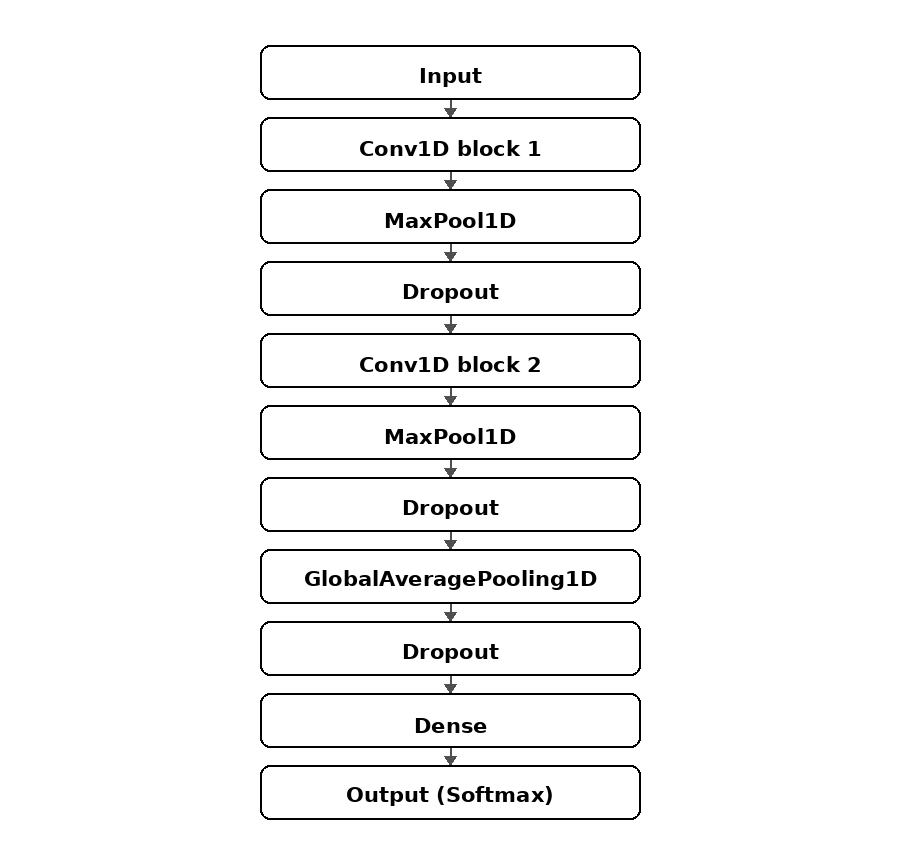
\includegraphics[width=0.8\textwidth]{obrazky-figures/nn_architecture.png}
  \caption{Baseline 1D-CNN architecture.}
  \label{fig:baseline_arch}
\end{figure}

 
\subsection{Training }
\label{sec:training}

The neural network is trained on windowed time-series data, where each sample consists of a fixed-length segment of IMU signals with the corresponding class label. The data are divided into training, validation, and test sets using a session-level split, ensuring that data from the same subject does not appear in multiple partitions.

Training is performed using the Adam optimizer with sparse categorical cross-entropy loss. The model is trained in mini-batches, and its performance is evaluated on the validation set after each epoch. Training runs for up to 50 epochs, with early stopping applied based on validation accuracy (patience of 8 epochs). This prevents overfitting and ensures that the model with the best validation performance is selected. The corresponding weights are restored at the end of training and used for final evaluation on the test set. The learning rate is treated as a tunable parameter and is varied across experiments.

After training, the selected model is converted to TensorFlow Lite format using\\ 
tf.lite.TFLiteConverter~\cite{litert}. To evaluate the trade-off between accuracy, memory usage, and computational efficiency, three quantization modes are considered: a float32 reference model, dynamic range quantization, and full int8 quantization. 

\subsection{Export, Quantization, and Firmware Deployment}
\label{sec:export}
 
The converted TFLite binary is embedded into the firmware as a static C byte array compiled directly into flash, eliminating any filesystem dependency. The per-channel normalization constants $\mu_c$ and $\sigma_c$ from training are compiled into a separate C header, ensuring that the runtime normalization on the microcontroller is numerically identical to the training normalization.
 
The firmware runs under FreeRTOS on the NXP i.MX RT1050, developed with MCUXpresso IDE and the NXP SDK. A button task handles debouncing and toggles recognition on and off. Sensor data is read from the MPU6050 using an interrupt-driven approach: the task polls the \texttt{INT\_STATUS} register of the MPU6050 and reads a new sample only when the data-ready bit is set, ensuring that samples are consumed at exactly the sensor's output data rate. The sensor task is scheduled using \texttt{vTaskDelayUntil} to maintain a regular execution period matching the sensor ODR.

Incoming sensor samples are stored in six circular buffers, one for each IMU channel. Before inference, each channel is normalized using precomputed mean and standard deviation values. For the int8 model, the normalized data are additionally quantized according to the model parameters. The prepared input is then passed to the TFLite Micro interpreter for prediction.

Inference time is measured by reading the ARM DWT cycle counter (a hardware register on Cortex-M processors that increments once per CPU clock cycle) and converted to time based on the processor frequency. After inference, the class with the highest softmax output is taken as the prediction. When the predicted class changes relative to the previous window, the class name and latency are printed over UART at 115200\,baud.

\section{Implementation Challenges}
\label{sec:challenges}
 
Several problems were encountered during implementation that influenced the final design decisions.
 
The accelerometer was initially configured with a full-scale range of $\pm$4\,g, which proved insufficient for fast wrist gestures. During sharp swipes the acceleration exceeded this limit and the output values were clipped at the maximum representable value, distorting the signal shape. Increasing the range to $\pm$8\,g eliminated the clipping and produced undistorted recordings across all gesture classes.
 
Sensor sampling was initially implemented by polling at a fixed FreeRTOS tick interval. Because FreeRTOS task scheduling is not cycle-accurate, the actual sampling interval varied slightly between ticks, causing inconsistent window boundaries and introducing jitter into the time-series data. Switching to interrupt-driven reading via the MPU-6050 INT pin ensured samples were consumed at exactly 50\,Hz regardless of other firmware activity.
 
An early evaluation used a random window-level train/test split. This produced inflated accuracy because adjacent windows from the same recording session appeared in both training and test partitions, making the evaluation optimistic. Switching to the session-level holdout split described in Section~\ref{sec:splitting} produced lower but honest accuracy estimates.
 

\chapter{Experimental Results and Analysis}
\label{chap:results}
% Analyzes trade-offs between accuracy, latency, and memory usage.

This chapter presents all experimental results. The first part reports the UCI HAR pipeline validation and parameter study (Section~\ref{sec:uci_results}). The second part covers gesture recognition experiments on the custom dataset, including model comparisons, quantization, and confidence thresholding (Section~\ref{sec:gesture_results}). The third part reports the cross-subject generalisation test (Section~\ref{sec:cross_subject}). The final section covers real-time deployment on the target board and models latency (Section~\ref{sec:realtime}).

\section{UCI HAR Parameter Study}
\label{sec:uci_results}

The UCI HAR dataset~\cite{anguita2013uci} contains recordings from 30 subjects performing six activity classes: walking, walking upstairs, walking downstairs, sitting, standing, and lying. The dataset provides a fixed cross-subject split of 21 training and 9 test subjects. These experiments isolate individual hyperparameter effects before applying the findings to the smaller gesture dataset. The baseline neural network configuration is given in Table~\ref{tab:baseline}. 
 
\begin{table}[ht]
  \centering
  \caption{Baseline 1D-CNN configuration for UCI HAR experiments.}
  \label{tab:baseline}
  \begin{tabular}{ll}
    \toprule
    \textbf{Parameter}    & \textbf{Value} \\
    \midrule
    Filters               & 32, 64 \\
    Kernel sizes          & 5, 3 \\
    Max pooling           & size~2 \\
    Dense layer           & 32 units, ReLU \\
    Dropout               & 0.2 \\
    Batch normalization   & disabled \\
    L2 regularization     & $10^{-3}$ \\
    Batch size            & 64 \\
    Epochs                & 100 \\
    Learning rate         & 0.001 \\
    \bottomrule
  \end{tabular}
\end{table}
 
\subsection{Effect of Filter Count}

Four filter configurations were evaluated. As shown in Table~\ref{tab:uci_filters}, more filters give better accuracy, but the improvement becomes smaller with each step. The gap between 8/16 and 16/32 is 11.1 percentage points, whereas the gap between 32/64 and 64/128 is only 1.3 points. As can be seen in Figure~\ref{fig:uci_filters}, the locomotion classes (walking, walking upstairs, walking downstairs) are classified reliably in all configurations. The static posture classes — sitting, standing, and lying — are the main source of error. This asymmetry is caused by the nature of the sensor signals. Locomotion activities produce strong, periodic patterns that are easy to detect even with a small number of filters. In contrast, static postures result in nearly constant signals that differ only in device orientation and small variations. Distinguishing between these classes requires the model to detect fine differences in signal baseline and low-amplitude variation, which demands more learned feature combinations than locomotion detection. With only 8/16 filters, the model does not have sufficient capacity to represent these distinctions; increasing filter count beyond 32/64 adds little discriminative power while increasing the model size.

\label{sec:uci_filters}
 
\begin{figure}[H]
  \centering
  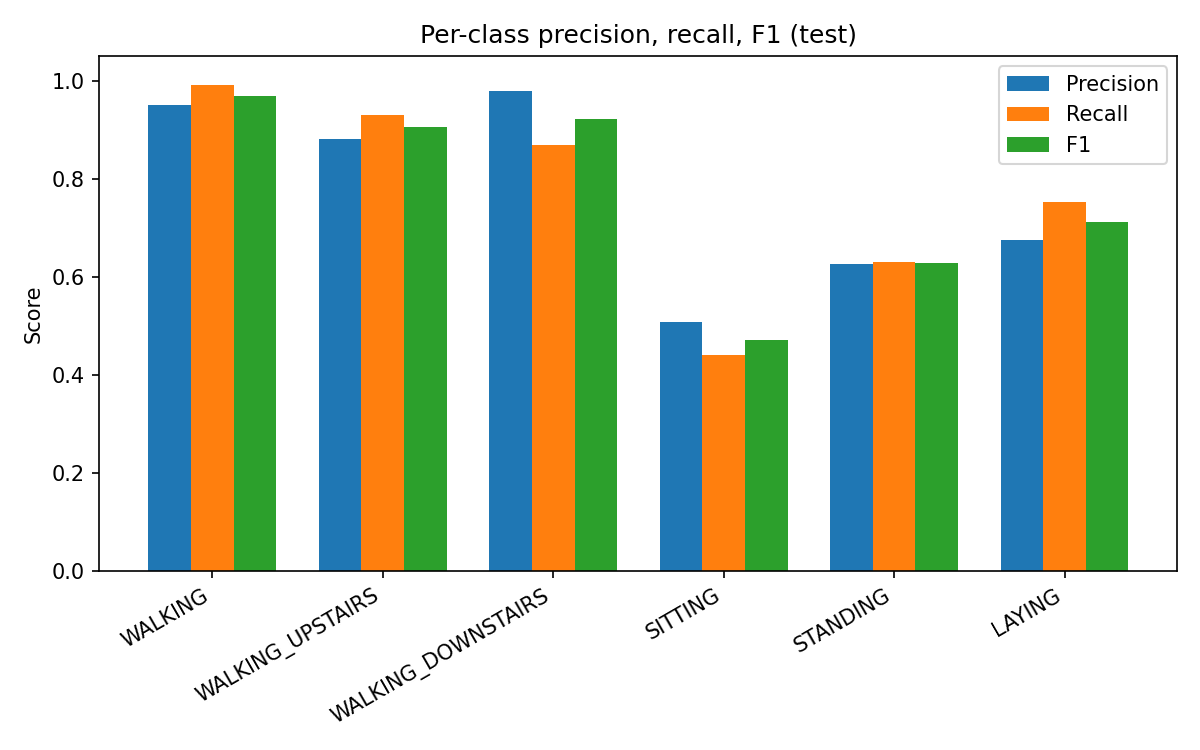
\includegraphics[width=0.8\textwidth]{obrazky-figures/uci_exp4_per_class.png}
  \hfill
  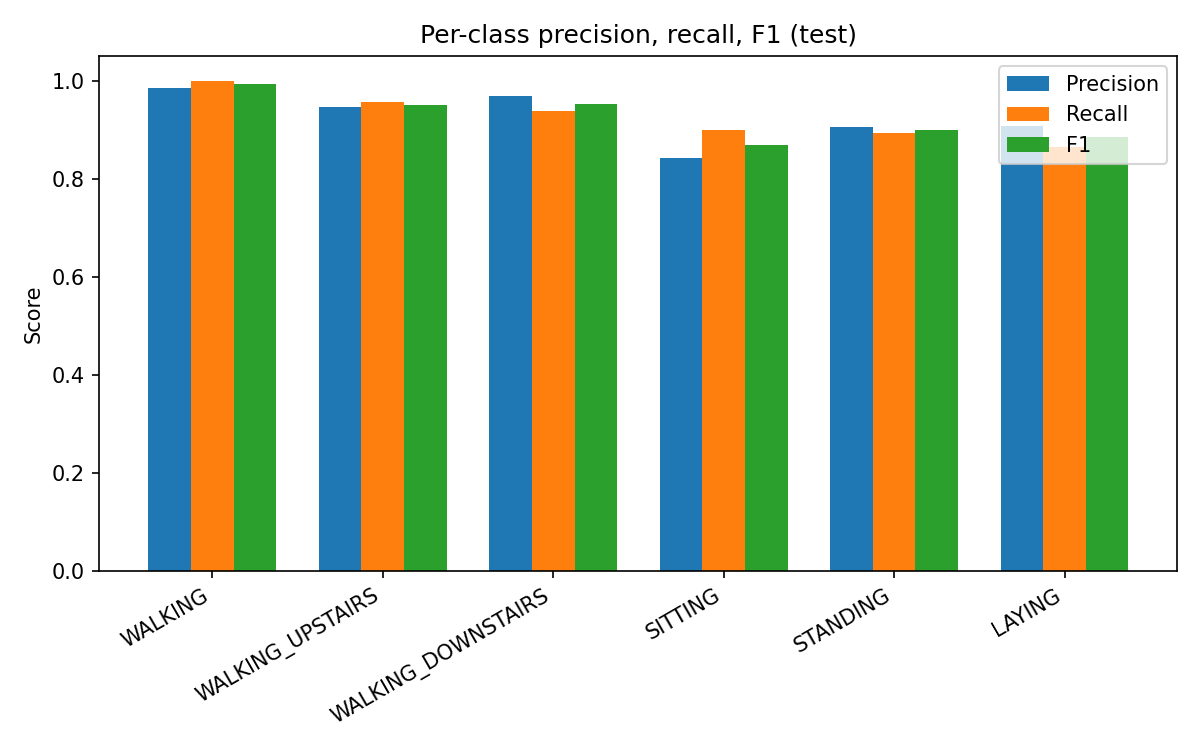
\includegraphics[width=0.8\textwidth]{obrazky-figures/uci_exp3_per_class.png}
  \caption{Per-class precision, recall, and F1-score for each of the six UCI HAR activity classes. Top panel: smallest filter configuration (8/16 filters, 76.3\% accuracy). Bottom panel: largest filter configuration (64/128 filters, 92.3\% accuracy).}
  \label{fig:uci_filters}
\end{figure}

\begin{table}[H]
  \centering
  \caption{Effect of convolutional filter count on UCI HAR.}
  \label{tab:uci_filters}
  \begin{tabular}{lrrr}
    \toprule
    \textbf{Filters} & \textbf{Test acc.} & \textbf{F1 macro}
      & \textbf{F1 weighted} \\
    \midrule
    8,  16   & 76.3\% & 0.768 & 0.763 \\
    16, 32   & 87.4\% & 0.877 & 0.874 \\
    32, 64   & 91.0\% & 0.913 & 0.912 \\
    64, 128  & 92.3\% & 0.925 & 0.923 \\
    \bottomrule
  \end{tabular}
\end{table}

The 76.3--92.3\% accuracy range across filter configurations on UCI is consistent with published results for comparable architectures~\cite{fawaz2019tsc}, confirming the pipeline implementation is correct.
 
\subsection{Effect of Dropout Rate and Learning Rate}
\label{sec:uci_dropout_lr}

Without dropout, the model reaches 92\% accuracy, slightly above baseline, because 21 training subjects already provide enough variety to prevent overfitting, so extra regularization is not needed. Increasing dropout to 0.6 causes a large drop to 69.8\% accuracy: deactivating 60\% of activations per step prevents the network from integrating information across both convolutional blocks, which is necessary to distinguish the six activity classes. On the gesture dataset, the same rate costs only 0.3 percentage points, more in Section~\ref{sec:gesture_reg}.

\begin{table}[ht]
  \centering
  \caption{Test accuracy and F1 macro on UCI HAR for different dropout rates.}
  \label{tab:uci_dropout}
  \begin{tabular}{lrr}
    \toprule
    \textbf{Dropout rate} & \textbf{Test acc.} & \textbf{F1 macro} \\
    \midrule
    0.0  & 92.0\% & 0.923 \\
    0.2  & 91.0\% & 0.913 \\
    0.6  & 69.8\% & 0.698 \\
    \bottomrule
  \end{tabular}
\end{table}

Table~\ref{tab:uci_lr} summarises the learning rate experiments. At LR $= 0.01$, accuracy drops slightly to 88.8\%, but at LR $= 0.0001$ the result is near-failure at 68.4\%: the model updates its weights too slowly and does not learn meaningful patterns within 100 epochs. As shown in Figure~\ref{fig:uci_lr_cm}, locomotion classes are still recognized reasonably well, but static posture classes collapse, with most samples predicted as a single class. This indicates that the model learns only the simplest distinction (locomotion versus static) without capturing finer differences. The learning rate is too low, so weight updates are limited, and training progresses slowly. The interesting point here is that on the gesture dataset, 0.0001 is the best learning rate, not a failing one. This contradiction is explained in detail in Section~\ref{sec:gesture_lr}.
 
\begin{table}[H]
  \centering
  \caption{Test accuracy and F1 macro on UCI HAR (6 classes) for different learning rates.}
  \label{tab:uci_lr}
  \begin{tabular}{lrr}
    \toprule
    \textbf{Learning rate} & \textbf{Test acc.} & \textbf{F1 macro} \\
    \midrule
    0.01    & 88.8\% & 0.891 \\
    0.001   & 91.0\% & 0.913 \\
    0.0001  & 68.4\% & 0.668 \\
    \bottomrule
  \end{tabular}
\end{table}

\begin{figure}[H]
  \centering
  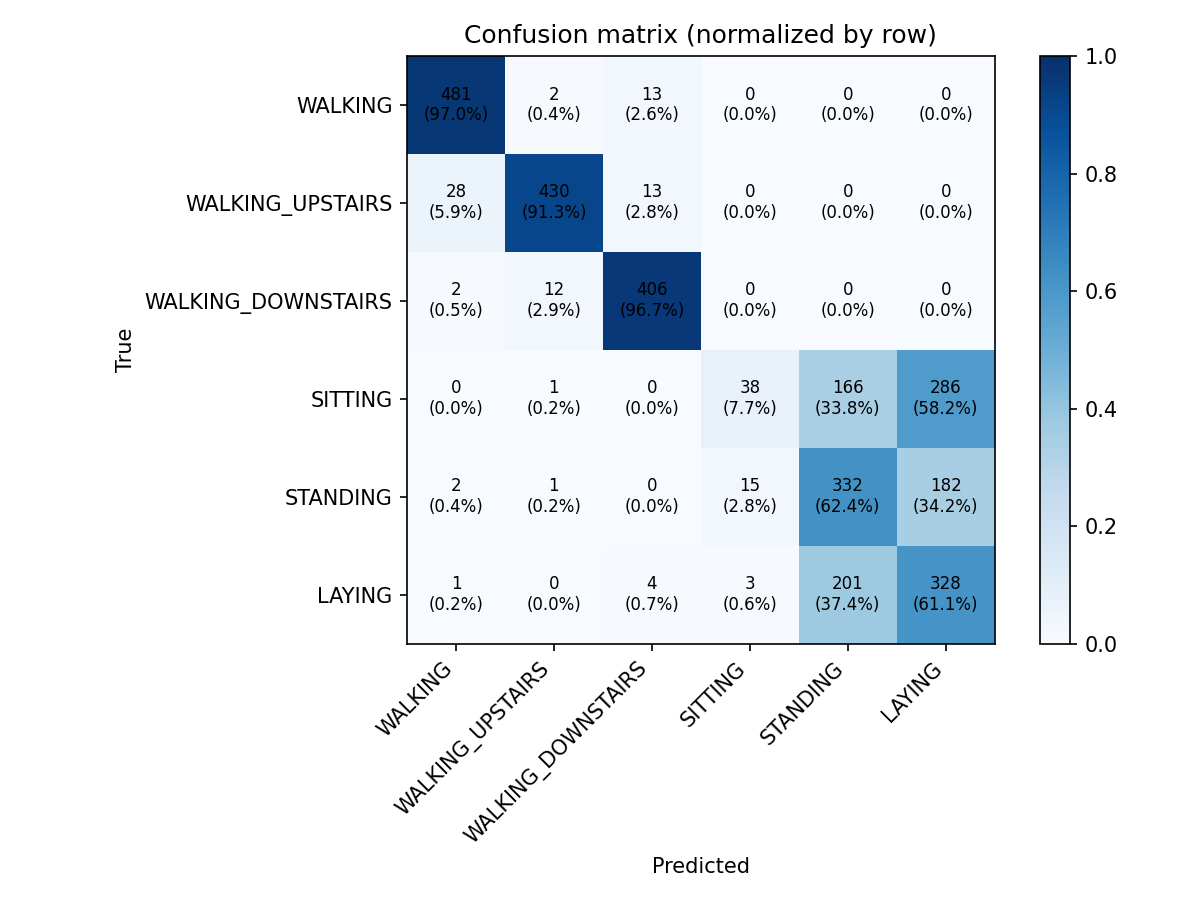
\includegraphics[width=0.9\textwidth]{obrazky-figures/uci_exp8_cm.png}
  \caption{Confusion matrix for the UCI HAR six-class task with learning rate 0.0001 (near-failure: 68.4\% test accuracy).}
  \label{fig:uci_lr_cm}
\end{figure}

\subsection{Effect of Batch Normalization}
\label{sec:uci_window_bn}
 
Adding batch normalization to the baseline reduces accuracy to 85.4\%. This seems surprising at first because batch normalization usually helps with training stability. The explanation is that batch normalization removes some of the natural variation in activations between different subjects. When the model is trained on multiple subjects and tested on unseen subjects, some of that inter-subject variation is exactly what the model needs to learn in order to generalize. Removing it during training produces a model that generalizes poorly to new individuals. This behavior is documented in the activity recognition literature and is particularly pronounced in datasets with large between-subject variability, such as UCI HAR. By contrast, on the small gesture dataset, batch normalization helps by stabilizing training on limited data.
 
 
\subsection{Classical Model Comparison on UCI}
\label{sec:uci_classical}
 
Table~\ref{tab:uci_classical} presents the results of the five classical classifiers on UCI HAR evaluated on the fixed test split. Figure~\ref{fig:uci_classical_comparison} shows the algorithm comparison bar chart.

Random forest achieves the highest accuracy at 86.6\%, followed by logistic regression at 82.2\%. The gap between the best classical model and the best CNN configuration, 64/128 filters at 92.3\%, is 5.7 percentage points. All classical models struggle with the static posture classes — sitting, standing, and laying — for the same reason as the low-filter CNN: the 30-dimensional feature vector does not capture sufficient orientation and periodicity information to reliably separate postures that differ only in body position rather than movement intensity. The kNN model shows the largest gap of 19.2 points compared to CNN, since the Euclidean distance in 30-dimensional space is a poor measure of similarity for the given class structure.
 
\begin{table}[ht]
  \centering
  \caption{Test accuracy, precision macro, and recall macro for five classical classifiers on the UCI HAR.}
  \label{tab:uci_classical}
  \begin{tabular}{lrrr}
    \toprule
    \textbf{Model} & \textbf{Test acc.} & \textbf{Precision macro} & \textbf{Recall macro} \\
    \midrule
    Random Forest       & 86.6\% & 0.867 & 0.866 \\
    Logistic Regression & 82.2\% & 0.823 & 0.822 \\
    SVM (Linear)        & 79.2\% & 0.793 & 0.792 \\
    Decision Tree       & 75.5\% & 0.756 & 0.755 \\
    k-NN ($k = 3$)      & 73.1\% & 0.731 & 0.731 \\
    \bottomrule
  \end{tabular}
\end{table}
 
\begin{figure}[ht]
  \centering
  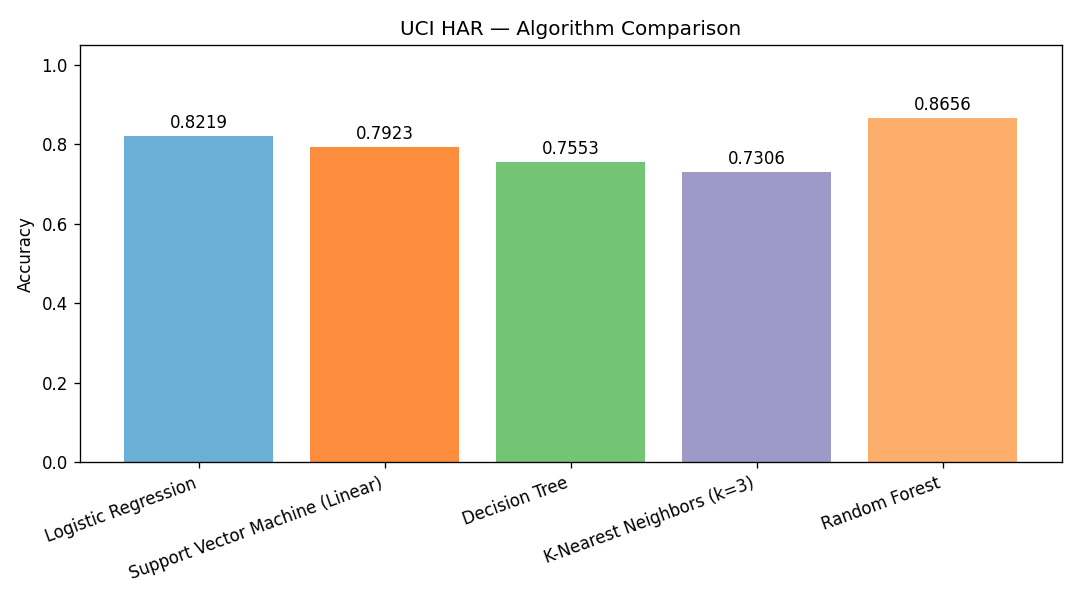
\includegraphics[width=0.95\textwidth]{obrazky-figures/uci_classical_comparison.png}
  \caption{Test accuracy of all five classical classifiers on the UCI HAR fixed test split.}
  \label{fig:uci_classical_comparison}
\end{figure}

\clearpage 
\section{Gesture Recognition Experiments}
\label{sec:gesture_results}

This section presents the experimental results for the five-class gesture dataset. The baseline configuration is given in Table~\ref{tab:baseline_gesture}. 
 
\begin{table}[H]
  \centering
  \caption{Baseline 1D-CNN configuration for gesture recognition experiments.}
  \label{tab:baseline_gesture}
  \begin{tabular}{ll}
    \toprule
    \textbf{Parameter}    & \textbf{Value} \\
    \midrule
    Filters               & 32, 64 \\
    Kernel sizes          & 5, 3 \\
    Max pooling           & size~2  \\
    Dense layer           & 32 units, ReLU \\
    Dropout               & 0.4 \\
    Batch normalization   & enabled \\
    L2 regularization     & $10^{-3}$ \\
    Batch size            & 64 \\
    Epochs                & 50 \\
    Learning rate         & 0.0001 \\
    Window / stride       & 100 samples / 50 samples \\
    \bottomrule
  \end{tabular}
\end{table}


\subsection{Baseline Performance}
\label{sec:gesture_baseline}

The baseline 1D-CNN achieves \textbf{94.3\%} test accuracy with F1 macro 0.943. Figure~\ref{fig:baseline_cm} shows the confusion matrix and~\ref{fig:baseline_roc} ROC curves.

\begin{figure}[ht]
  \centering
    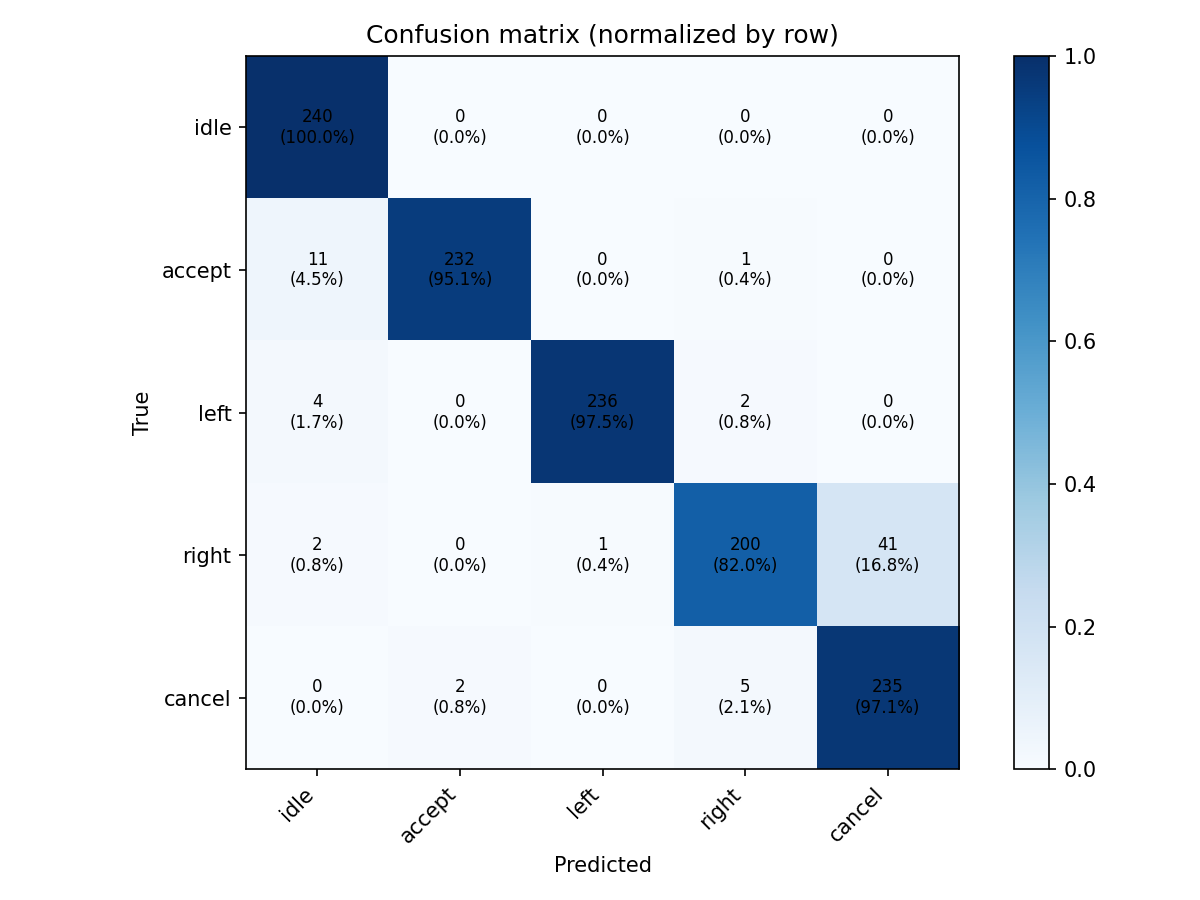
\includegraphics[width=0.85\textwidth]{obrazky-figures/gesture_exp1_cm.png}
    \caption{Confusion matrix for the baseline 1D-CNN on the five-class gesture dataset.}
    \label{fig:baseline_cm}
\end{figure}

\begin{figure}[H]
    \centering
    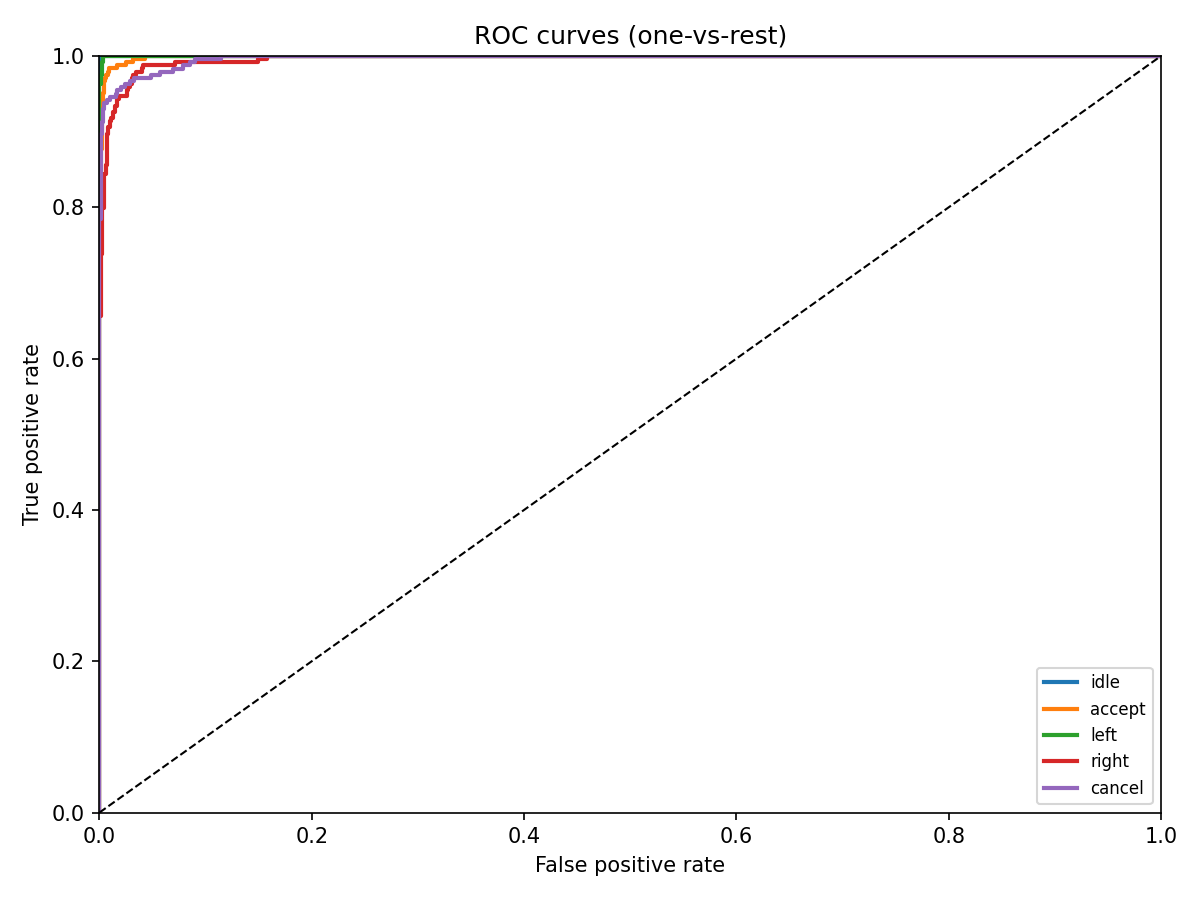
\includegraphics[width=0.8\textwidth]{obrazky-figures/gesture_exp1_roc.png}
    \caption{ROC curves (one-vs-rest strategy) for the baseline 1D-CNN on the five-class gesture test set. }
    \label{fig:baseline_roc}
\end{figure}

Idle reaches 100\% recall, left 97.5\%, cancel 97.1\%, accept 95.1\%. The right class is most difficult at 82.0\% recall, with 16.8\% misclassified as cancel. This confusion has a clear physical explanation. Both subjects are right-handed, and the return movement at the end of a rightward swipe produces a leftward deceleration that is similar to the onset of the cancel wrist shake. This overlap is present in all training data, so the model cannot learn to separate them reliably without more subjects or a redesigned gesture vocabulary.

\subsection{Effect of Filter Count on Gesture Data}
\label{sec:gesture_filters}

For the gesture dataset, reducing the filter count is not only about accuracy but also about how much memory the model needs on the microcontroller. Table~\ref{tab:gesture_filters} shows both dimensions together.

\begin{table}[ht]
  \centering
  \caption{Accuracy and memory footprint for different filter counts on the
           gesture dataset.}
  \label{tab:gesture_filters}
  \begin{tabular}{lrrrr}
    \toprule
    \textbf{Filters} & \textbf{Test acc.} & \textbf{F1 macro}
      & \textbf{Flash (B)} & \textbf{RAM (B)} \\
    \midrule
    8,  16  & 86.9\% & 0.865 & 11\,132 &  37\,716 \\
    16, 32  & 92.5\% & 0.924 & 18\,844 &  72\,692 \\
    32, 64  & 94.3\% & 0.943 & 43\,484 & 151\,860 \\
    \bottomrule
  \end{tabular}
\end{table}

Halving the filters from 32/64 to 16/32 costs 1.8 percentage points of accuracy while reducing RAM by more than half. Reducing further to 8/16 filters gives 86.9\% accuracy with only 37\,716 bytes of RAM. This configuration would fit even on a Cortex-M4 device with 128\,KB SRAM. But at 8/16, the confusion shifts from right/cancel to right/left, indicating a qualitatively different and worse decision boundary.

\begin{figure}[H]
  \centering
  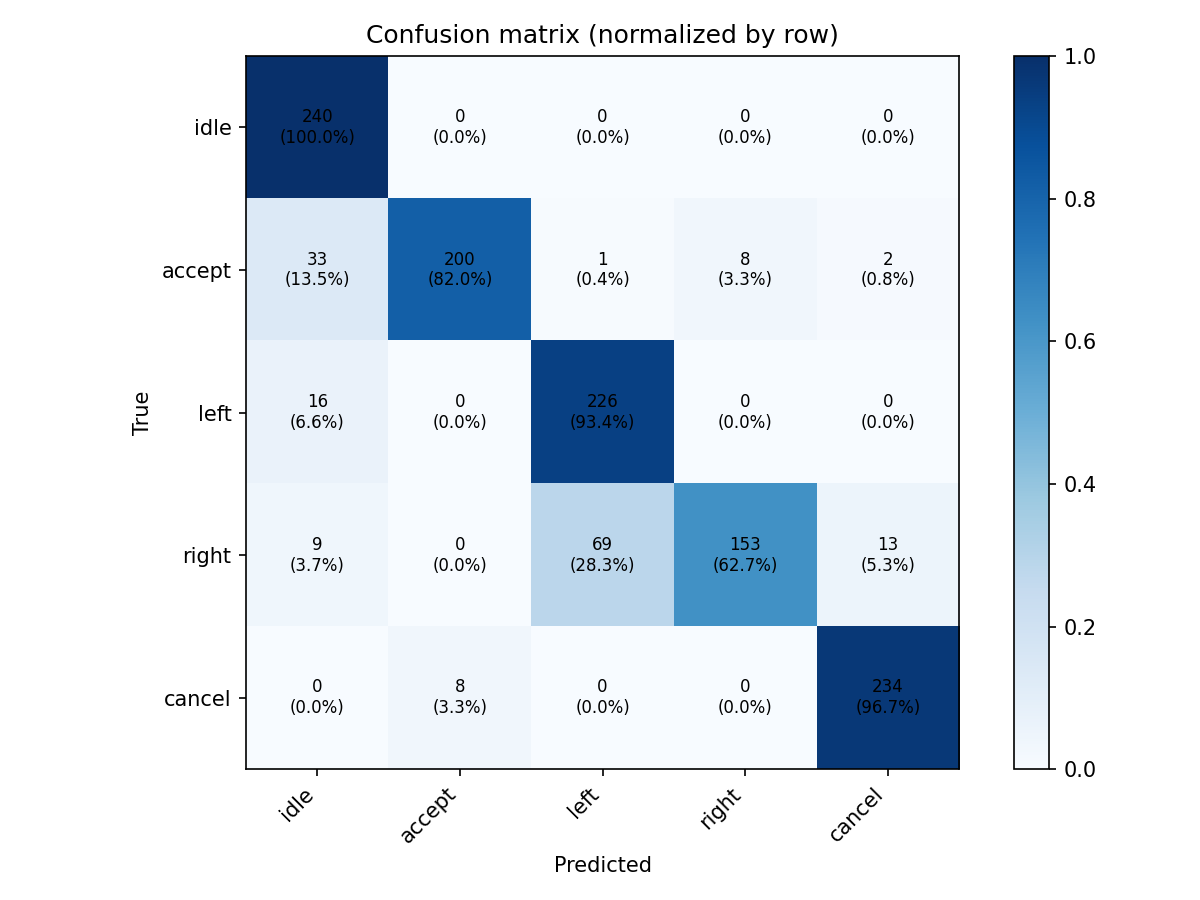
\includegraphics[width=0.8\textwidth]{obrazky-figures/gesture_cm_8.png}
  \caption{Confusion matrix for the filter configuration 8/16 on the gesture dataset.}
  \label{fig:gesture_window_cm_8}
\end{figure}

The offline accuracy gap between 16/32 and 32/64 is modest, but live deployment testing revealed a more pronounced difference in behavior. The 16/32 model showed more frequent misclassifications on the right and cancel classes, while the 32/64 configuration handled this ambiguous transition more reliably. Since confusion between right and cancel can lead to incorrect system actions, the additional 79 KB of RAM required by the larger model was considered acceptable. Both configurations fit within the available memory, so the 32/64 model was selected for further experiments and deployment.

\subsection{Effect of Learning Rate on Gesture Data}
\label{sec:gesture_lr}

Table~\ref{tab:gesture_lr} shows the results for different learning rates on the gesture dataset. The baseline learning rate of 0.0001 gives the best result. Increasing to 0.01 reduces accuracy to 93.6\% and changes the confusion pattern in the accept class: 10.2\% of accept samples are now misclassified as right. Reducing the learning rate to 0.000001 causes complete failure at 20.0\%, near random chance for five classes, because the weight updates are so small that the model cannot move away from its random initialization within 50 training epochs.

\begin{table}[H]
  \centering
  \caption{Test accuracy and F1 macro on the gesture dataset for different learning rates.}
  \label{tab:gesture_lr}
  \begin{tabular}{lrr}
    \toprule
    \textbf{Learning rate} & \textbf{Test acc.} & \textbf{F1 macro} \\
    \midrule
    0.01      & 93.6\% & 0.936 \\
    0.0001    & 94.3\% & 0.943 \\
    0.000001  & 20.0\% & 0.090 \\
    \bottomrule
  \end{tabular}
\end{table}

As noted earlier in Section~\ref{sec:uci_dropout_lr}, the learning rate 0.0001 causes near-failure on UCI, but it is optimal there. With 21 training subjects, each epoch provides a more informative gradient signal, which supports faster parameter updates. In contrast, with only two subjects, the gradient signal is weaker, so each epoch contributes less information. A smaller learning rate is therefore more appropriate, as it reduces the risk of overshooting the minimum when training on limited data.

\subsection{Effect of Dropout, Regularization, and Batch Normalization}
\label{sec:gesture_reg}

Removing dropout gives 95.3\% test accuracy, slightly above the baseline. However, the validation accuracy reaches exactly 1.0 from around epoch 30, which is a sign of overfitting. The model has memorized the training sessions rather than learning general gesture patterns, so it would likely perform worse on new subjects. Increasing dropout to 0.6 gives 94.6\%, essentially the same as the baseline, while train accuracy is only 83.5\%. Because the training data have low diversity, the two-subject dataset is relatively simple, and even strong dropout does not prevent the model from learning. This is very different from the UCI results (Section~\ref{sec:uci_dropout_lr}), where the same dropout rate caused a drop of about 20 percentage points. This shows that the choice of regularization depends on how large and diverse the training data are.

\begin{table}[ht]
  \centering
  \caption{Test accuracy on the gesture dataset for different dropout rates and regularization settings. }
  \label{tab:gesture_dropout}
  \begin{tabular}{lrr}
    \toprule
    \textbf{Configuration} & \textbf{Test acc.} & \textbf{F1 macro} \\
    \midrule
    Dropout 0.0              & 95.3\% & 0.953 \\
    Dropout 0.4 (baseline)   & 94.3\% & 0.943 \\
    Dropout 0.6              & 94.6\% & 0.946 \\
    \addlinespace
    No batch normalization   & 94.0\% & 0.940 \\
    No L2 regularization     & 94.6\% & 0.946 \\
    \bottomrule
  \end{tabular}
\end{table}

\begin{figure}[H]
  \centering
  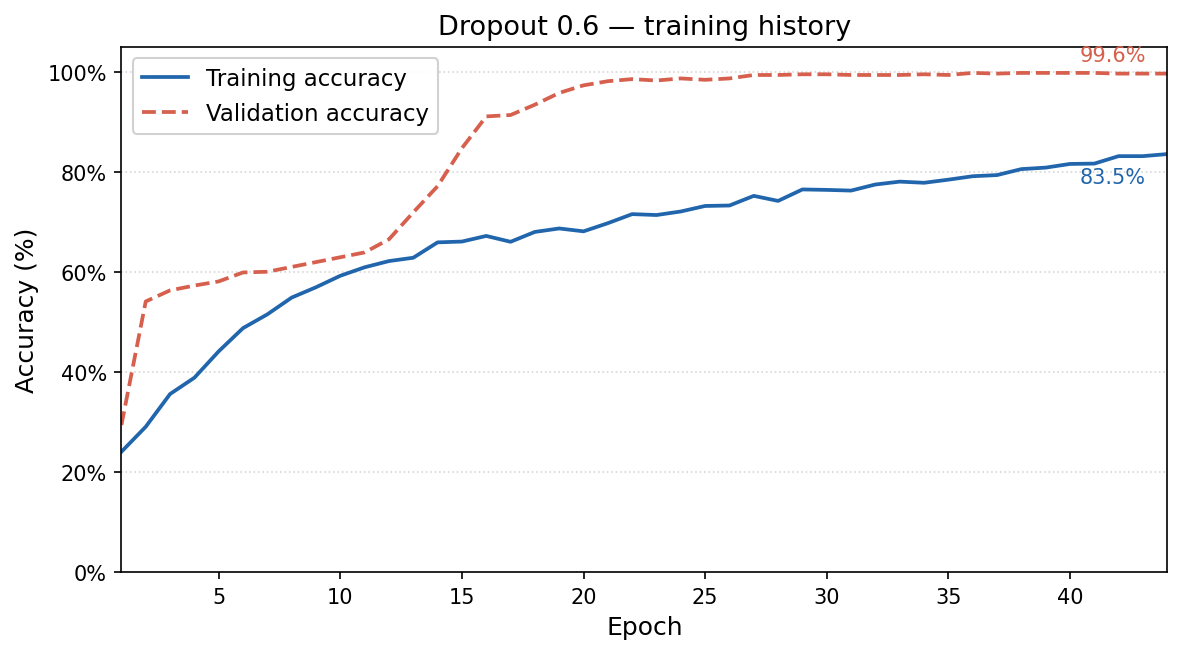
\includegraphics[width=0.8\textwidth]{obrazky-figures/gesture_dropout_history.png}
  \caption{Training accuracy and validation accuracy per epoch on the gesture dataset with dropout rate 0.6.}
  \label{fig:gesture_dropout}
\end{figure}

Removing batch normalization gives 94.0\%, and removing L2 regularization gives 94.6\%. The small changes indicate that, on this relatively uniform dataset, both techniques have
only a minor individual effect. Their main benefit is stabilizing training in the early epochs when the gradient from two subjects is noisy.

\subsection{Effect of Window and Stride}
\label{sec:gesture_window}

Table~\ref{tab:gesture_window} compares different window and stride settings. Increasing the stride while keeping the window at 100 samples consistently reduces accuracy. With no overlap at all (stride 100), accuracy drops to 91.0\% because fewer and less varied training windows are generated from each recording. Overlapping windows create more training examples and make the model less sensitive to where exactly a gesture starts within a window.

\begin{table}[h]
  \centering
  \caption{Test accuracy, F1 macro, and SRAM consumption for different window sizes and stride lengths on the gesture dataset.}
  \label{tab:gesture_window}
  \begin{tabular}{lrrrr}
    \toprule
    \textbf{Window} & \textbf{Stride} & \textbf{Test acc.}
      & \textbf{F1 macro} & \textbf{RAM (B)} \\
    \midrule
    100 & 100 & 91.0\% & 0.906 & 151\,860 \\
    100 &  75 & 92.3\% & 0.921 & 151\,860 \\
    100 &  50 & 94.3\% & 0.943 & 151\,860 \\
    200 & 100 & 96.2\% & 0.962 & 265\,460 \\
    \bottomrule
  \end{tabular}
\end{table}

Using a 200-sample window with a stride 100 gives the best result across all 15 gesture experiments: 96.2\% accuracy with F1 macro 0.962. At 50\,Hz, a four-second window captures the complete gesture motion, including the return phase; right recall improves from 82.0\% to 86.0\%, and cancel reaches 100\%.

\begin{figure}[H]
  \centering
  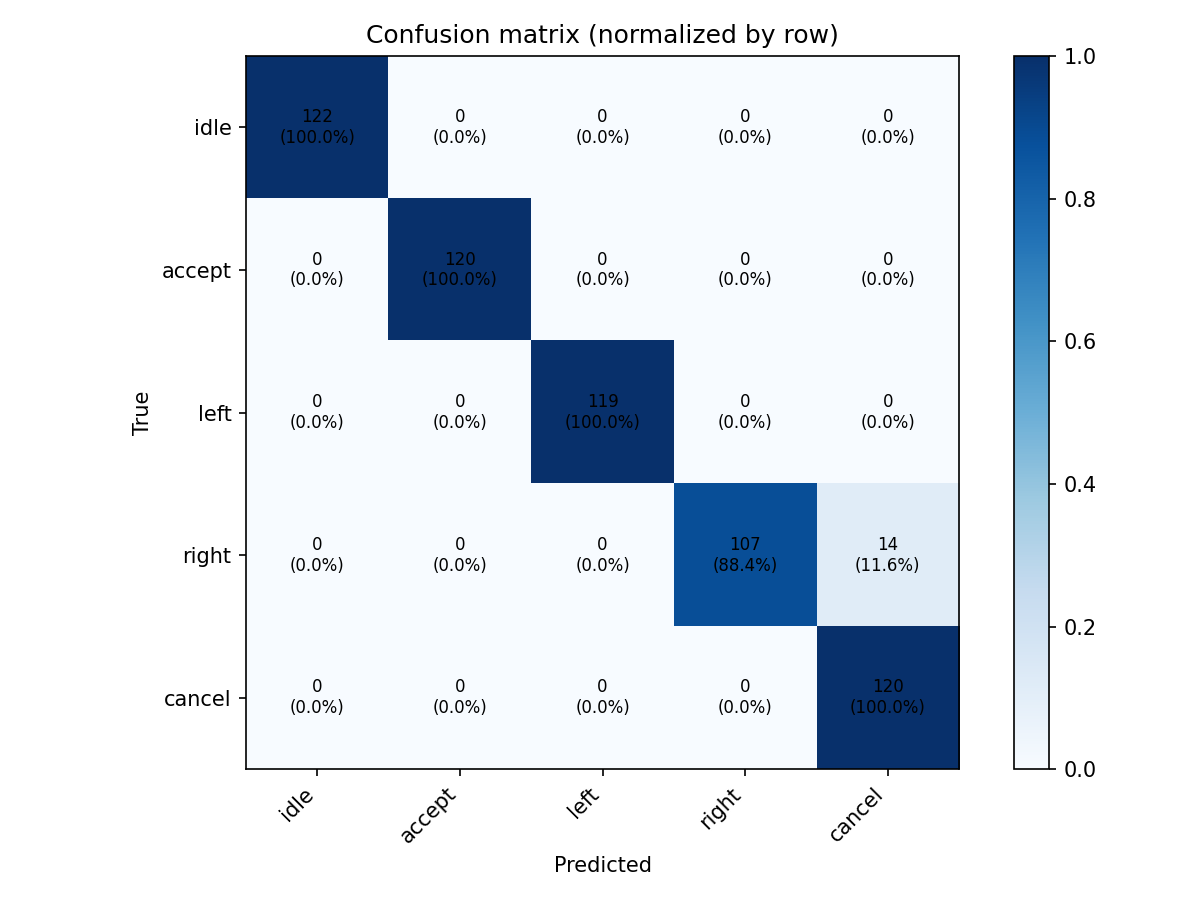
\includegraphics[width=0.80\textwidth]{obrazky-figures/gesture_exp13_cm.png}
  \caption{Confusion matrix for the best window setting (window 200, stride 100).}
  \label{fig:gesture_window_cm}
\end{figure}

However, the larger window introduces a noticeable delay during live inference that was not present with the 100-sample baseline. Because the firmware triggers inference only after a full 200-sample window has accumulated, and the stride is 100 samples, a new prediction becomes available every two seconds at 50\,Hz. In practice, this means the user sometimes has to perform the gesture twice before the correct class is detected reliably. This delay is not visible in the offline accuracy numbers, which is an important reminder that high test accuracy does not automatically translate to smooth real-time behavior. For applications where response time matters more than maximum accuracy, the 100-sample baseline is the better practical choice despite its lower offline score.

The larger window also needs more RAM: 265\,460 bytes compared to 151\,860 for the baseline. Both values are well within the 512\,KB SRAM of the NXP i.MX RT1050. On a more limited device such as a Cortex-M4 with 128\,KB SRAM, the baseline window would be the only viable option on both memory and latency grounds.

\subsection{Quantization Results}
\label{sec:quantization}

As shown in Table~\ref{tab:quantization}, full int8 quantization reduces SRAM by 75\% — from 151\,860 to 38\,406 bytes — and flash from 43\,484 to 19\,512 bytes, with only a $+0.4$ percentage point accuracy change. Dynamic range quantization gives a marginally higher accuracy (95.4\%), likely due to the mild regularization effect of quantization noise, but saves less RAM since activations remain in float32. 

The int8 model uses about 7.3\% of the available 512\,KB SRAM on the i.MX RT1050, leaving plenty of space for the FreeRTOS kernel, task stacks, UART buffers, and any other application data. Full int8 quantization is the right choice for this deployment: the accuracy loss is minimal, and the memory savings are very large.

\begin{table}[ht]
  \centering
  \caption{Test accuracy, F1 macro, flash consumption, and SRAM consumption for three quantization modes of the baseline gesture model.}
  \label{tab:quantization}
  \begin{tabular}{lrrrr}
    \toprule
    \textbf{Configuration} & \textbf{Test acc.} & \textbf{F1 macro}
      & \textbf{Flash (B)} & \textbf{RAM (B)} \\
    \midrule
    Float32 (no quantization) & 94.3\% & 0.943 & 43\,484 & 151\,860 \\
    Dynamic range             & 95.4\% & 0.953 & 20\,144 & 127\,284 \\
    Full int8                 & 94.7\% & 0.947 & 19\,512 &  38\,406 \\
    \bottomrule
  \end{tabular}
\end{table}

\subsection{Confidence Thresholding}
\label{sec:thresholding}

The training script also evaluates how the model behaves when a confidence threshold is applied: predictions where the highest softmax output is below a threshold $\tau$ are rejected rather than passed on. Figure~\ref{fig:threshold} shows how coverage (the fraction of predictions that are accepted) and accuracy on accepted predictions change as the threshold increases.

At $\tau = 0$, all predictions are accepted, and accuracy equals the test accuracy of 94.3\%. As the threshold increases, the model rejects low-confidence predictions, so accuracy on what remains improves while coverage falls. At the threshold of $\tau \approx 0.5$, almost all predictions are still accepted, but their accuracy rises to about 97\%. 

Most low-confidence predictions come from confusion between the right and cancel classes, because the model is uncertain at the boundary between these gestures. Applying a threshold in the firmware would therefore reduce the errors that are most problematic in real use, while having almost no effect on coverage.

\begin{figure}[H]
  \centering
  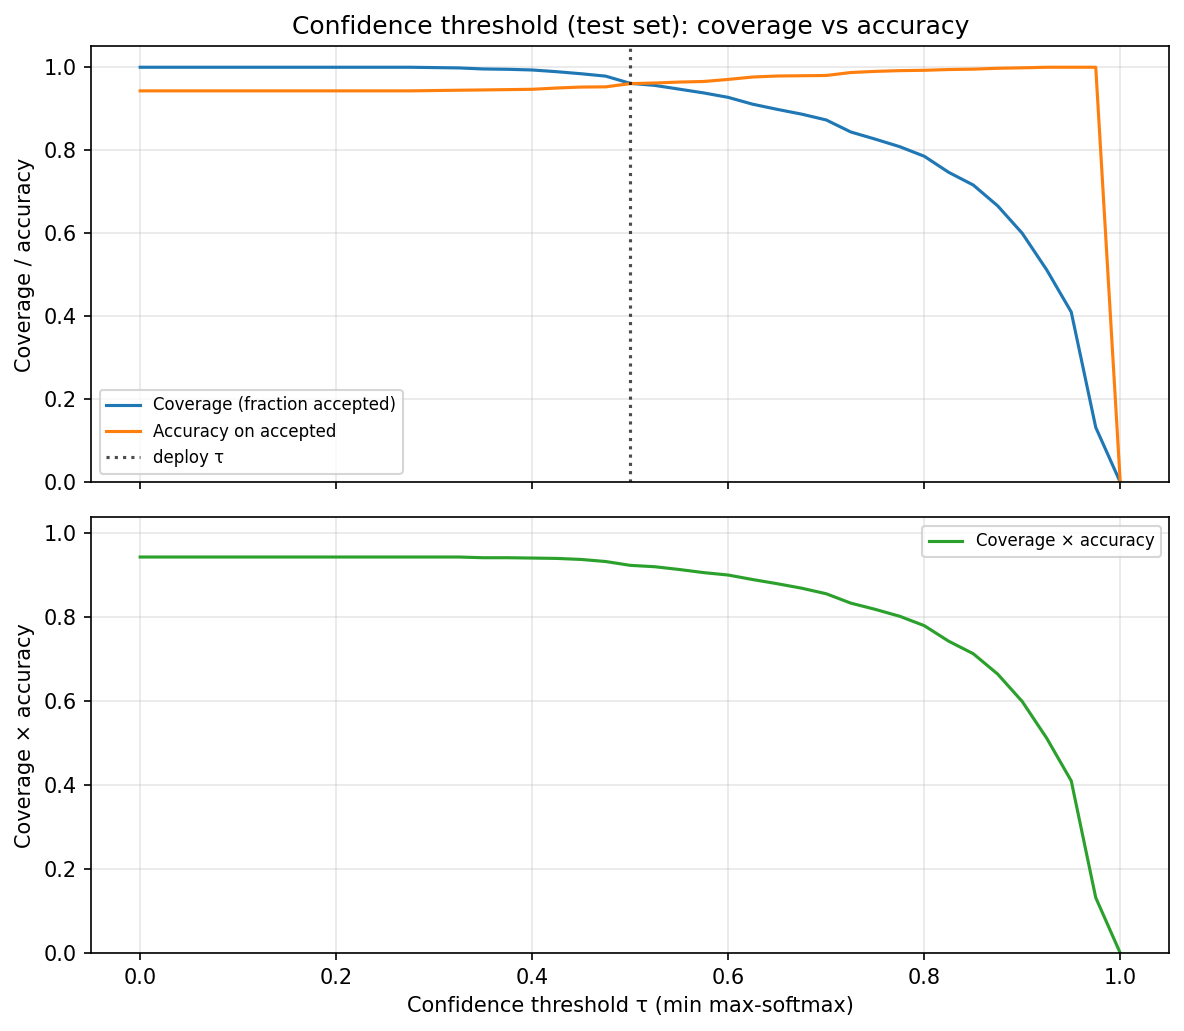
\includegraphics[width=0.85\textwidth]{obrazky-figures/gesture_exp1_treshhold.png}
  \caption{Confidence threshold analysis for the baseline gesture model.}
  \label{fig:threshold}
\end{figure}

\subsection{Classical Model Comparison on Gesture Data}
\label{sec:gesture_classical}

Table~\ref{tab:gesture_classical} shows the results of the five classical models on the gesture dataset, both on the single test split and under five-fold group cross-validation; figure~\ref{fig:gesture_classical_comparison} gives a visual overview.

Logistic regression achieves 96.1\% on the single test split, matching the best 1D-CNN result. Under cross-validation, kNN leads at 93.4\% while the decision tree shows the highest variance ($\pm0.114$), which means its performance depends heavily on which sessions end up in the test fold.

\begin{table}[ht]
  \centering
  \caption{Test accuracy on the single session holdout split and five-fold group cross-validation accuracy (mean ± std across folds) for five classical classifiers on the gesture dataset. }
  \label{tab:gesture_classical}
  \begin{tabular}{lrr}
    \toprule
    \textbf{Model} & \textbf{Test acc. (split)}
      & \textbf{CV accuracy (mean $\pm$ std)} \\
    \midrule
    Logistic Regression    & 96.1\% & $0.898 \pm 0.082$ \\
    k-NN ($k = 3$)         & 94.7\% & $0.934 \pm 0.057$ \\
    Random Forest          & 92.3\% & $0.906 \pm 0.091$ \\
    SVM (Linear)           & 91.4\% & $0.893 \pm 0.083$ \\
    Decision Tree          & 91.4\% & $0.835 \pm 0.114$ \\
    \bottomrule
  \end{tabular}
\end{table}

\begin{figure}[ht]
  \centering
  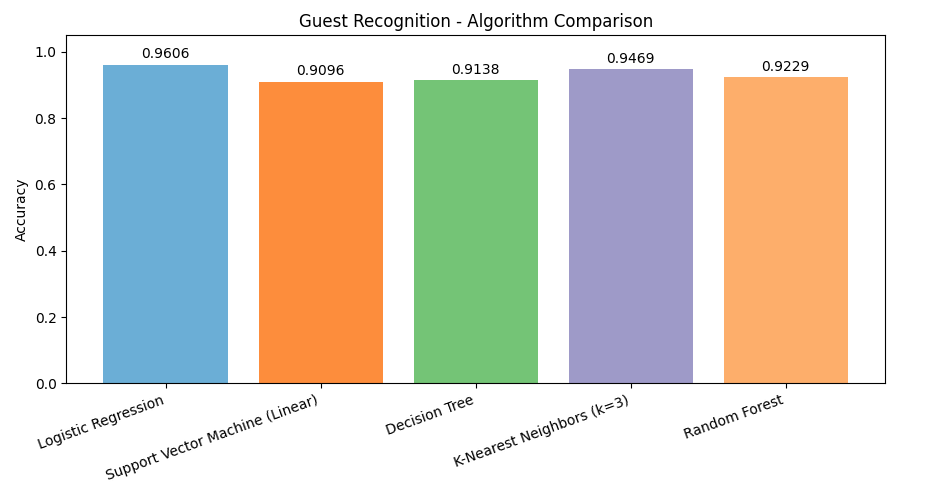
\includegraphics[width=0.9\textwidth]{obrazky-figures/guesture_classical_comparison.png}
  \caption{Test accuracy of all five classical models on the gesture dataset.}
  \label{fig:gesture_classical_comparison}
\end{figure}

Good classical model performance on a small dataset is a well-known pattern. With only two subjects and five sessions each, the training set is small enough that a simple linear classifier can find the main boundaries without needing the representational depth of a neural network. The advantage of the CNN becomes visible only with more data, which the UCI results confirm: on UCI, the CNN consistently outperforms all classical models.

\section{Cross-Subject Generalization}
\label{sec:cross_subject}
All results above measure within-subject generalization. To find out whether the model can work with someone completely new, one additional experiment was run: the model was trained only on Subject~B's four sessions per class and tested on Subject~A's held-out session. 

The test accuracy is \textbf{34.7\%}, which is only slightly higher than the 20\% expected from random chance for five classes — combined with a test loss of 1.63, indicates that the model produces confident but incorrect predictions: the characteristic signature of subject-specific overfitting. 

The cancel class achieves 99.2\% recall, but this is not a sign of generalization — it means the model redirects most ambiguous predictions from other classes toward cancel. The per-class chart confirms the severity of the failure~\ref{fig:cross_subject_char}. The ROC curves show that cancel and accept perform well, while left and right are near or below random. The idle curve stays around 0.5 TPR, indicating random performance~\ref{fig:cross_subject_roc}. 

This result is not a failure of the model architecture. It is the expected consequence of training on one person. The MPU6050 captures fine-grained wrist kinematics that naturally differ between individuals in resting orientation, joint angles, motion amplitude, and gesture speed. A model trained on one person learns these personal characteristics as if they were part of the gesture definition. When applied to Subject~A, the decision boundaries built around Subject~B's personal kinematics do not match, and the model fails on the classes where individual variation is largest.

\begin{table}[ht]
  \centering
  \caption{Within-subject vs.\ cross-subject generalization of the baseline 1D-CNN.}
  \label{tab:generalization}
  \begin{tabular}{lcccc}
    \toprule
    \textbf{Evaluation} & \textbf{Test acc.} & \textbf{Test loss} \\
    \midrule
    Within-subject (session holdout) & 94.3--96.2\% & $<0.3$ \\
    Cross-subject (unseen person)    & 34.7\%        & 1.63 \\
    \bottomrule
  \end{tabular}
\end{table}

\begin{figure}[H]
    \centering
    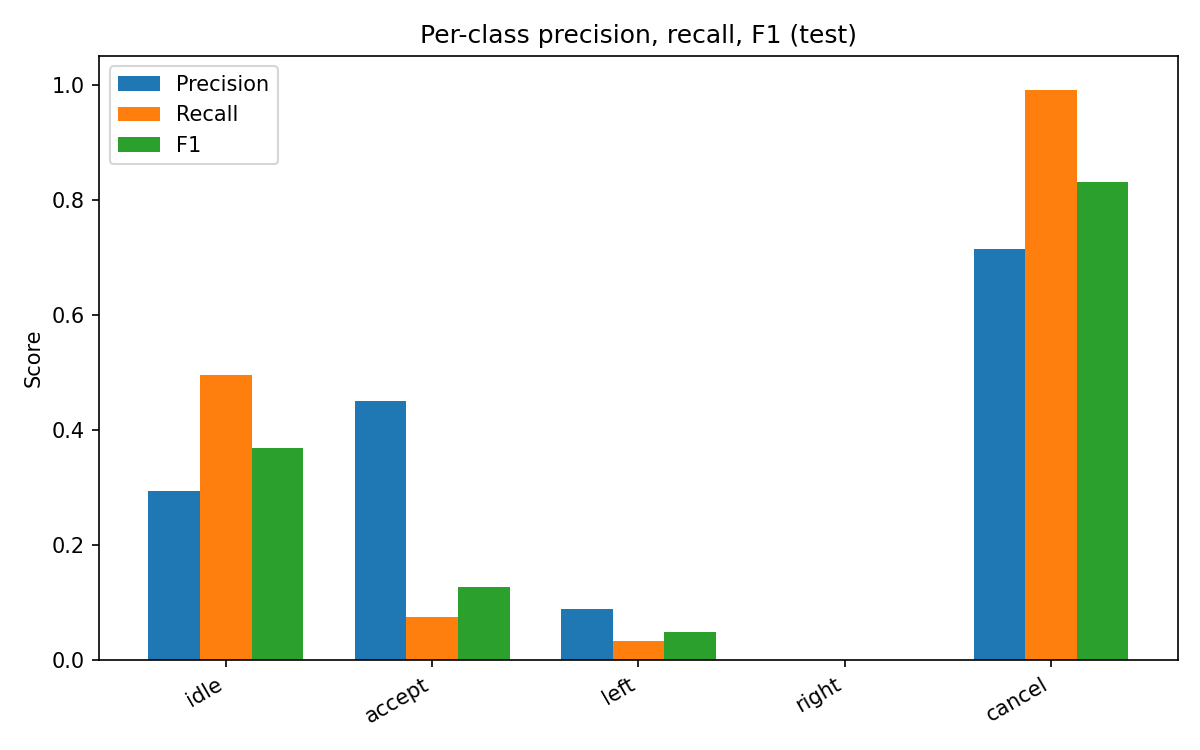
\includegraphics[width=0.80\textwidth]{obrazky-figures/gesture_cross_subject_per_class.png}
    \caption{Per-class precision, recall, and F1-score for the cross-subject experiment.}
    \label{fig:cross_subject_char}
\end{figure}

\begin{figure}[H]
    \centering
    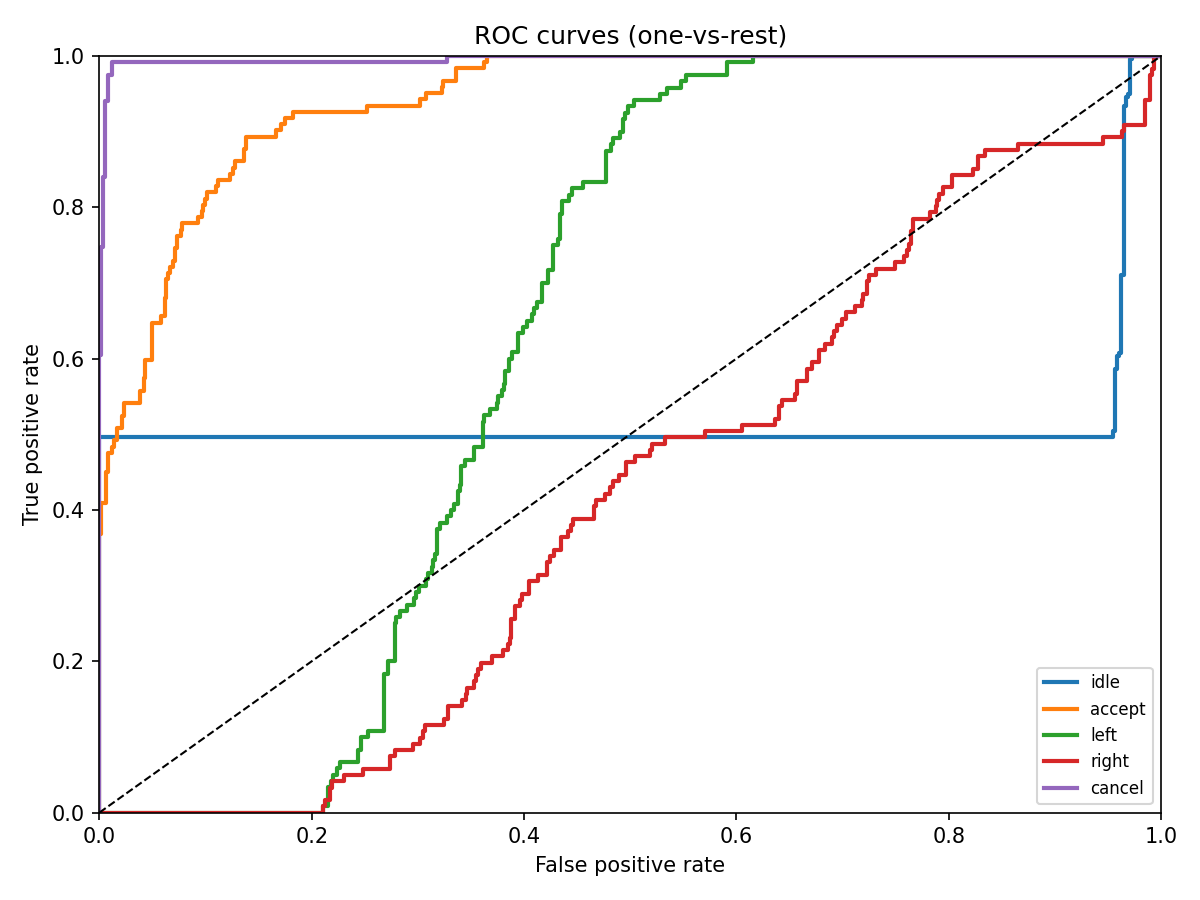
\includegraphics[width=0.75\textwidth]{obrazky-figures/gesture_cross_subject_roc.png}
    \caption{ROC curves (one-vs-rest) for the cross-subject experiment.}
    \label{fig:cross_subject_roc}
\end{figure}

The system, as trained, is therefore reliable only for the subjects who contributed data. Deployment to a wider user base would require either collecting personalized training data for each new user or substantially expanding the subject pool during initial training.

\section{Real-Time Inference on the Target Board}
\label{sec:realtime}

Three classical models and quantization variants of the 1D-CNN were deployed on the NXP i.MX RT1050 and tested during live gesture recognition. Inference time and end-to-end latency were measured using the ARM DWT cycle counter as described in Section~\ref{sec:export}. Table~\ref{tab:latency_all} summarises the measured results for all deployed models.

\begin{table}[ht]
  \centering
  \caption{Measured on-board inference latency and flash footprint for all deployed models (window 100 samples, stride 50 samples, sensor ODR 50\,Hz).}
  \label{tab:latency_all}
  \small
  \begin{tabular}{lrrrr}
    \toprule
    \textbf{Model} & \textbf{Avg inf ($\mu$s)} & \textbf{Max inf ($\mu$s)}
      & \textbf{Avg lat ($\mu$s)} & \textbf{Flash (B)} \\
    \midrule
    Logistic regression  & 584 & 595 & 587 & 620 \\
    Linear SVM           & 584 & 595 & 587 & 620 \\
    Decision tree        & 221 & 232 & 224 & 9\,756 \\
    Random Forest        & 3\,721 & 5\,010 & 3\,725 & 1\,465\,680 \\
    1D-CNN float32       & 28\,518 & 38\,687 & 28\,522 & 43\,484 \\
    1D-CNN int8          & 13\,199 & 23\,737 & 13\,203 & 19\,512 \\
    \bottomrule
  \end{tabular}
\end{table}

\subsection{Neural Network Inference Latency}

With a stride of 50 samples at 50\,Hz, a new window becomes available every 1000\,ms. The average inference time for int8 is 13,199\,$\mu$s while for float32 it is 28,518\,$\mu$s; both leave significant headroom—the processor spends less than 2\% of the available budget on inference.

The first inference in each session takes longer; this is a one-time cache warm-up effect. The ARM Cortex-M7 has a 16\,KB instruction cache and a 16\,KB data cache; the first pass through the model loads the TFLite Micro kernel code and model weights into cache. All subsequent inferences are performed from the cache and achieve stable latency within the second window. Enabling CMSIS-NN integer kernels gives int8 a \textbf{2.2$\times$ speedup} over float32 at steady state. 

Both models are deployable in real time on this platform. The int8 model is the better choice for deployment because it is 2.2$\times$ faster, uses 75\% less RAM (38,406 vs approximately 150,000 bytes at runtime), and reduces flash from 43,484 to 19,512 bytes with only 0.4 percentage points of accuracy loss.

\subsection{Classical Model Latency}

The decision tree is the fastest deployed model at 221\,$\mu$s average, using 9\,756 bytes of flash for its node arrays. Logistic regression and linear SVM both measure 584\,$\mu$s — both values are dominated by the feature extraction step rather than the model inference itself, since computing mean, MAD, min, max, and ZCR across six channels per 100-sample window accounts for the majority of cycles. The actual matrix-vector multiply requires only a few hundred operations.

The average response time of the random forest is 3\,721\,$\mu$s with a maximum of 5\,010\,$\mu$s. This is significantly longer than the three single-model classifiers because inference requires traversing all 120 trees independently and aggregating their majority vote. The latency also shows greater variability than any other deployed model: the minimum observed was approximately 3\,070\,$\mu$s and the maximum 5\,010\,$\mu$s, a spread of roughly 63\%. This variability arises because different input windows activate different branch paths across the ensemble — active gesture windows with higher feature variation tend to reach deeper leaves before resolving, while idle windows converge faster. In terms of latency, the random forest remains within the 1000\,ms inference budget and is approximately 3.5 times faster than the int8 CNN. However, its flash footprint is significantly larger at 1\,465\,680 bytes, occupying around 70\% of the i.MX RT1050’s internal flash memory. While the model can still be deployed on the target platform, its memory requirements would become problematic on more constrained microcontrollers.

The decision tree, logistic regression, and linear SVM are comfortably deployable on microcontrollers with much greater limitations than the i.MX RT1050. In terms of latency, all four classical models occupy less than 0.4\% of the available inter-window interval.

\subsection{Observed Prediction Behavior}

The following observations are based on live testing with the models deployed on the NXP i.MX RT1050. All models printed their predictions to the PC terminal via UART in real time, which made class transitions directly observable.
 
\paragraph{1D-CNN.}
The CNN classified idle reliably when the hand was held in a natural resting position with the wrist pointing downward. When the wrist was held in a raised or horizontal position between gestures, the model frequently predicted accept instead of idle, because the static sensor orientation in that posture resembles the beginning of the accept gesture. After the hand remained stationary for a few seconds in that position, the model corrected itself and settled on idle, indicating that the temporal context accumulated across subsequent windows was sufficient to resolve the ambiguity. Among the active gesture classes, left was occasionally misclassified as right and right as cancel, both of which are consistent with the confusion patterns observed in the offline results and explained by kinematic overlap at the gesture boundaries. Overall, the number of sustained wrong predictions was low, and most errors were transient.
 
\paragraph{Classical models.}
All four classical models exhibited the same error patterns as the CNN, but more frequently. Wrong class predictions occurred more often, particularly at gesture onset and offset, and the models switched between class labels more rapidly during transitions. This instability arises from the feature-based inference mechanism: statistical features such as mean and ZCR computed over a single 100-sample window can change significantly from one window to the next during a transition, causing abrupt prediction changes that the CNN, which processes the full raw time-series, handles more smoothly. The idle misclassification in raised-wrist postures was also present in all four classical models and resolved similarly over time.
 
This difference in temporal stability is not visible in the offline accuracy results, which measure predictions for each window separately and do not consider consistency over time. In real applications, where each class change produces a visible or audible response, this instability would be noticeable to the user. For this reason, the CNN is more suitable for deployment, in addition to its higher accuracy.

\chapter{Conclusion}
\label{chap:conclusion}
% Summarizes main experimental outcomes.
The goal of this thesis was to investigate whether a compact machine learning model can be trained, optimized, and deployed on a microcontroller-based embedded system for real-time gesture recognition, and to evaluate how the choice of model architecture, hyperparameters, and quantization mode affects the resulting system's accuracy, memory footprint, and
inference latency. 
 
The implemented system successfully recognizes five wrist gesture classes from raw IMU data in real time on the NXP~i.MX~RT1050. The baseline 1D-CNN achieved 94.3\% test accuracy within a session-based holdout evaluation, rising to 96.2\% with a longer input window. After full int8 quantization, the SRAM footprint dropped by 75\% -- from 151\,860 to 38\,406 bytes -- and flash by 55\%, with an accuracy change of only $+0.4$ percentage points. The int8 model completes inference in 13\,199~$\mu$s on average, spending under 2\% of the 1000~ms inter-window budget, which confirms that real-time operation on this platform is feasible with substantial headroom remaining. Classical models were also deployed successfully: the decision tree completes inference in 221~$\mu$s using under 10~KB of flash, and logistic regression matches the best CNN accuracy on the gesture dataset in offline evaluation. However, live deployment testing showed that the CNN produced slightly more stable predictions across consecutive windows, making it the preferred choice for real-time use.

The UCI hyperparameter study served two purposes. The primary one was to validate the training pipeline on a dataset with a known published baseline before applying it to the custom gesture data, where an implementation error would be much harder to detect. The results matched published values for this benchmark, which confirmed the pipeline was correct. The study also produced a useful secondary observation: the optimal values of learning rate, dropout, and batch normalization are not the same for the two datasets, and for several parameters, the direction of the effect reverses between UCI and the gesture data. This is not a dataset-specific anomaly but a consequence of gradient signal quality: with 21 training subjects, each epoch provides a diverse and informative gradient, supporting faster and more aggressive optimization, while with only two subjects, the gradient is weaker and noisier, requiring slower and more careful updates. 
 
The comparison of the 1D-CNN and classical models across both datasets confirmed the expected pattern: the CNN outperforms classical models on the large UCI benchmark, while on the small gesture dataset classical models perform competitively and offer significant advantages in memory footprint and inference time. This finding supports the conclusion that the choice between a neural network and a classical classifier for embedded deployment should be driven primarily by the amount of available training data and the specific resource constraints of the target platform.

The work has several limitations worth noting. The most significant is the two-subject training corpus. Cross-subject testing yielded only 34.7\,\% accuracy, showing that the system in its current form is personalized and does not generalize to new users without additional training data or an on-device enrolment step. 

A second limitation concerns the hardware scope: all latency and memory measurements were obtained on a single NXP~i.MX~RT1050 board. The quantization and filter count experiments show how model footprint changes with configuration, but a direct comparison across different microcontroller families would give a more complete picture of how the same model behaves under varying hardware constraints.

Several directions would extend and improve this work. Expanding the training corpus to more subjects is likely the most impactful step: even three to five additional participants would enable proper leave-one-subject-out cross-validation and would likely close most of the cross-subject accuracy gap. A practical near-term alternative is on-device personalization, where a new user performs a small number of gesture repetitions directly on the device and only the final dense layer is updated on this data, which is feasible within the available SRAM budget without modifying the model architecture.

Deploying the same quantized model on additional platforms~-- a Cortex-M4 device such as the Arduino Nano~33~BLE Sense and a platform with a hardware neural network accelerator such as the STM32H7 with Cube.AI support~-- would complete the platform comparison and provide concrete evidence of how inference latency and memory scale across the microcontroller design space.

  \else
    \input{projekt-01-kapitoly-chapters}
  \fi
  
  % Kompilace po částech (viz výše, nutno odkomentovat a zakomentovat input výše)
  % Compilation piecewise (see above, it is necessary to uncomment it and comment out input above)
  %\subfile{chapters/projekt-01-uvod-introduction}
  % ...
  %\subfile{chapters/projekt-05-zaver-conclusion}

  % Pouzita literatura / Bibliography
  % ----------------------------------------------
\ifslovak
  \makeatletter
  \def\@openbib@code{\addcontentsline{toc}{chapter}{Literatúra}}
  \makeatother
  \bibliographystyle{bib-styles/Pysny/skplain}
\else
  \ifczech
    \makeatletter
    \def\@openbib@code{\addcontentsline{toc}{chapter}{Literatura}}
    \makeatother
    \bibliographystyle{bib-styles/Pysny/czplain}
  \else 
    \makeatletter
    \def\@openbib@code{\addcontentsline{toc}{chapter}{Bibliography}}
    \makeatother
    \bibliographystyle{bib-styles/Pysny/enplain}
  %  \bibliographystyle{alpha}
  \fi
\fi
  \begin{flushleft}
  \bibliography{projekt-20-literatura-bibliography}
  \end{flushleft}

  % vynechani stranky v oboustrannem rezimu
  % Skip the page in the two-sided mode
  \iftwoside
    \cleardoublepage
  \fi

  % Prilohy / Appendices
  % ---------------------------------------------
  \appendix
\ifczech
  \renewcommand{\appendixpagename}{Přílohy}
  \renewcommand{\appendixtocname}{Přílohy}
  \renewcommand{\appendixname}{Příloha}
\fi
\ifslovak
  \renewcommand{\appendixpagename}{Prílohy}
  \renewcommand{\appendixtocname}{Prílohy}
  \renewcommand{\appendixname}{Príloha}
\fi
%  \appendixpage

% vynechani stranky v oboustrannem rezimu
% Skip the page in the two-sided mode
%\iftwoside
%  \cleardoublepage
%\fi
  
\ifslovak
%  \section*{Zoznam príloh}
%  \addcontentsline{toc}{section}{Zoznam príloh}
\else
  \ifczech
%    \section*{Seznam příloh}
%    \addcontentsline{toc}{section}{Seznam příloh}
  \else
%    \section*{List of Appendices}
%    \addcontentsline{toc}{section}{List of Appendices}
  \fi
\fi
  \startcontents[chapters]
  \setlength{\parskip}{0pt} 
  % seznam příloh / list of appendices
  % \printcontents[chapters]{l}{0}{\setcounter{tocdepth}{2}}
  
  \ifODSAZ
    \setlength{\parskip}{0.5\bigskipamount}
  \else
    \setlength{\parskip}{0pt}
  \fi
  
  % vynechani stranky v oboustrannem rezimu
  \iftwoside
    \cleardoublepage
  \fi
  
  % Přílohy / Appendices
  % \ifenglish
  %   \input{projekt-30-prilohy-appendices-en}
  % \else
  %   \input{projekt-30-prilohy-appendices}
  % \fi
  
  % Kompilace po částech (viz výše, nutno odkomentovat)
  % Compilation piecewise (see above, it is necessary to uncomment it)
  %\subfile{projekt-30-prilohy-appendices}
  
\end{document}
